\documentclass{scrbook}
%\hypersetup{colorlinks}% uncomment this line if you prefer colored hyperlinks (e.g., for onscreen viewing)
%% Check out the stuff commented with three %'s

\usepackage[margin=1.2in]{geometry}
\usepackage[english]{babel}
\usepackage[utf8]{inputenc}
\usepackage[T1]{fontenc}
\usepackage{lmodern}
\usepackage{amsmath}
\usepackage{graphicx}
%\usepackage{fancyhdr}
\usepackage{textcomp}
\usepackage{comment}
\usepackage[framemethod=tikz]{mdframed}
% \usepackage[pdftex,
%             pdfauthor={Prof. Vikram M. Gadre},
%             pdftitle={EE210.1X Lecture Notes},
%             pdfsubject={Signals and Systems}]{hyperref}
% \pagestyle{fancy}
% \lhead{IITBombayX}
% \rhead{EE210.1X}
%\cfoot{\thepage}
%\renewcommand{\headrulewidth}{0.4pt}
%\renewcommand{\footrulewidth}{0.4pt}

% Book metadata
\title{\Huge Signals and Systems}
\author{\Large Dr. Vikram Gadre}
%\publisher{Publisher of This Book}
%%%\usepackage{booktabs}
\usepackage{graphicx}
%%%\setkeys{Gin}{width=\linewidth,totalh.eight=\textheight,keepaspectratio}
\graphicspath{{graphics/}}
%
\newcommand{\blankpage}{\newpage\hbox{}\thispagestyle{empty}\newpage}
% Generates the index
\usepackage{makeidx}
\makeindex
\begin{document}

% Front matter
\frontmatter

% r.1 blank page
%\blankpage
% r.3 full title page
\maketitle

\begin{comment}
% v.4 copyright page
\newpage
\begin{fullwidth}
~\vfill
\thispagestyle{empty}
\setlength{\parindent}{0pt}
\setlength{\parskip}{\baselineskip}
Copyright \copyright\ \the\year\ \thanklessauthor

\par\smallcaps{Published by \thanklesspublisher}

\par\smallcaps{tufte-latex.googlecode.com}

\par Licensed under the Apache License, Version 2.0 (the ``License''); you may not
use this file except in compliance with the License. You may obtain a copy
of the License at \url{http://www.apache.org/licenses/LICENSE-2.0}. Unless
required by applicable law or agreed to in writing, software distributed
under the License is distributed on an \smallcaps{``AS IS'' BASIS, WITHOUT
WARRANTIES OR CONDITIONS OF ANY KIND}, either express or implied. See the
License for the specific language governing permissions and limitations
under the License.\index{license}

%\par\textit{First printing, \monthyear}
\end{fullwidth}
\end{comment}
% r.5 contents
\tableofcontents

\listoffigures

\listoftables

\begin{comment}
% r.7 dedication
\cleardoublepage
~\vfill
\begin{doublespace}
\noindent\fontsize{18}{22}\selectfont\itshape
\nohyphenation
Dedicated to those who appreciate \LaTeX{} 
and the work of \mbox{Edward R.~Tufte} 
and \mbox{Donald E.~Knuth}.
\end{doublespace}
\vfill
\vfill
\end{comment}

% r.9 introduction
\cleardoublepage
\mainmatter

\part{Frequency Domain}
\chapter{Sinusoids and LSI Systems}
\section{Module 2: Lecture 1\\Sinusoidal Signals and their Properties}

\subsection*{Introduction}
In the first module, we have been looking at signals and systems in what is
called their natural domain. By natural domain, we mean that the independent
variable of the signal is the same as it was when the signal was
recorded or observed or instituted. An example of a signal in its natural
domain is a speech signal expressed as a function of time, as time is the
naturally associated independent variable with the speech signal. \\
For processing signals, we need appropriate systems. Now, what processing needs to be done by the system can be a tricky thing to specify in the
natural domain. \\
For example, say we want to separate the voices of male and female
singers from an audio recording of a chorus. Although it is qualitatively easier to understand, one can't give the description of such a system in the
time domain. We need to
have a broader view of systems, and more importantly, of signals, to be able
to tackle this problem. \\
So in this module we are going to take the first step towards a change of
paradigm, a change of world-view in describing signals and systems.
%% Adding the Introduction from M2L02 here as of now.
In this lecture we will learn how to deal with phase changes in sinusoidal signals and pass sinusoidal signals into stable LSI systems in an intelligent and insightful manner. We will look into why we introduced complex signals in our previous analysis and how these tools make the mathematical modelling simple. We then go on to understanding how to deal with signals beyond the domain of sinusoids.
%% Intro of M2L02 ends here
We begin by understanding which signals are special from the point of view of
the signals and systems. Let's visit the ideal voltage generator for that
purpose.
\subsection{The Ideal Voltage generator}
The ideal voltage generator consists of a circular conducting coil rotating in
a constant magnetic field.
\begin{figure}[ht]
\centering
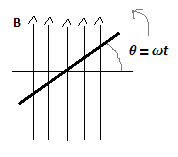
\includegraphics{flux.png}
\caption{\label VVoltage generator (side view)}
\end{figure}
\\
Let the area enclosed by the coil be $A$, the angular frequency of
rotation be $\omega$ such that $\theta = \omega t$, and the value of the
constant magnetic field be $B$. Now, by Faraday's law, the electric field $\mathcal{E}$ is defined as
\[ \mathcal{E}= - \frac{\partial \Phi_B}{\partial t} \]
where the flux $\Phi_B$ in this case is given by
\[ \Phi_B = BA \cos \theta = BA \cos \omega t \]
Hence the electric field will be
\[ \mathcal{E}= - BA \ \omega \sin \omega t \]
This is the principle of generation of the voltage supply that we receive at
our residences. This is one important reason why the sinusoidal voltage is
highly favoured and deeply studied. And of course there are many other reasons
why. Let us have a look at some interesting properties of sinusoids.
%%%
%%%
\subsection{Properties of sinusoids}
The first interesting thing about sine waves is that when you add two sinusoids
of the same frequency, it gives you back another sinusoid of the \emph{same}
frequency. Let's prove this formally.
Say we have two sinusoids, $x_1 (t)$ and $x_2 (t)$, of the same angular frequency
$\Omega,$ given by
\begin{equation*}
x_1 (t) = A_1 \cos (\Omega t + \phi_1)
\end{equation*}
\begin{equation*}
x_2 (t) = A_2 \cos (\Omega t + \phi_2)
\end{equation*}
Now consider a linear combination of the two sinusoids,
\begin{equation*}
x (t) = \alpha_1 x_1 (t) + \alpha_2 x_2 (t)
\end{equation*}
Note that we can write $x_1$ and $x_2$ as
\begin{equation*}
x_1 (t) = A_1  \{ \cos \Omega t \cos \phi_1 - \sin \Omega t \sin \phi_1 \}
\end{equation*}
\begin{equation*}
x_2 (t) = A_2  \{ \cos \Omega t \cos \phi_2 - \sin \Omega t \sin \phi_2 \}
\end{equation*}
Hence we can write $x (t)$ as
\begin{equation*}
x (t) = [ \alpha_1 A_1 \cos \phi_1 + \alpha_2 A_2 \cos \phi_2 ] \cos
   \Omega t + [ - \alpha_1 A_1 \sin \phi_1 - \alpha_2 A_2 \sin
   \phi_2 ] \sin \Omega t
\end{equation*}
Writing the two time-independent coefficients as $P$ and $Q$, we get
\begin{equation*}
 x (t) = P \cos \Omega t + Q \sin \Omega t = \sqrt{P^2 + Q^2}  \left\{
   \frac{P}{\sqrt{P^2 + Q^2}} \cos \Omega t + \frac{Q}{\sqrt{P^2 + Q^2}}
   \sin \Omega t \right\}
\end{equation*}
This can be easily seen to be
\begin{equation*}
 x (t) = \sqrt{P^2 + Q^2} \cos (\Omega t + \Phi)
\end{equation*}
with
\begin{equation*}
\Phi = - \tan^{- 1} \left( \frac{Q}{P} \right)
\end{equation*}
Hence, linearly combining two sinusoids of the same frequency gives back a
sinusoid with the same frequency.\\
Another interesting property is that when we differentiate a
sine wave, we get back a sinusoid of the same frequency.
\begin{equation*}
\frac{d}{d t}  \{ A \cos (\Omega t + \phi) \} = - A \Omega \sin
   (\Omega t + \phi)
\end{equation*}
It doesn't matter whether it is cosine or sine since they differ only by a
phase of $\pi / 2$.
\[ \cos (\Omega t + \phi) = \sin (\Omega t + \phi + \pi / 2) \]
Now let's see how we can describe a change in amplitude of a sinusoid.
Suppose the original sinusoid is given by
\[ x_1 (t) = A \cos (\Omega t + \phi) \]
and let the changed sinusoid is given by
\[ x_2 (t) = B \cos (\Omega t + \phi) \]
where $A$ and $B$ are positive constants. Then,
\[ x_2 (t) = \frac{B}{A} x_1 (t) \]
So the change of amplitude in a sinusoid is simply described by a multiplying
constant.\\
But this is not true for a phase change. Suppose the original sinusoid is
given by
\[ x_1 (t) = A \cos (\Omega t + \phi_1) \]
and the changed sinusoid is given by
\[ x_2 (t) = A \cos (\Omega t + \phi_2) \]
Unlike the amplitude case, $x_2 (t) / x_1 (t)$ doesn't turn out to be a
constant independent of time. This will cause a problem while dealing with
inductors or capacitors. In inductors, for example, the voltage drop is
proportional to the derivative of the current passing through it. Hence, if a
sinusoidal current is passing through it, the voltage drop across it will also
be a sinusoid, but will have a phase difference of $90^0$ with the current.
Hence, we cannot establish a relationship like the resistor $(V = RI)$ in case
of the inductor since $V / I$ won't be a constant independent of time.\\
To deal with this problem, we will have to use the rotating complex number
representation of the sinusoid.

\subsection{Sinusoids as Rotating Complex Numbers}

We can think of a sinusoid $I_0 \cos (\Omega t + \phi_0)$ as a combination of
two rotating complex numbers. Let the first begin at time $t = 0$ with an
angle of $\phi_0$. Let it have a magnitude of $I_0 / 2$ and let the other
begin with the same magnitude $I_0 / 2$ but the opposite starting angle ($-
\phi_0$). Let them both rotate with an angular velocity of $\Omega$, but the
first one in counter clockwise and the second one in clockwise direction.
\begin{figure}[ht]
\centering
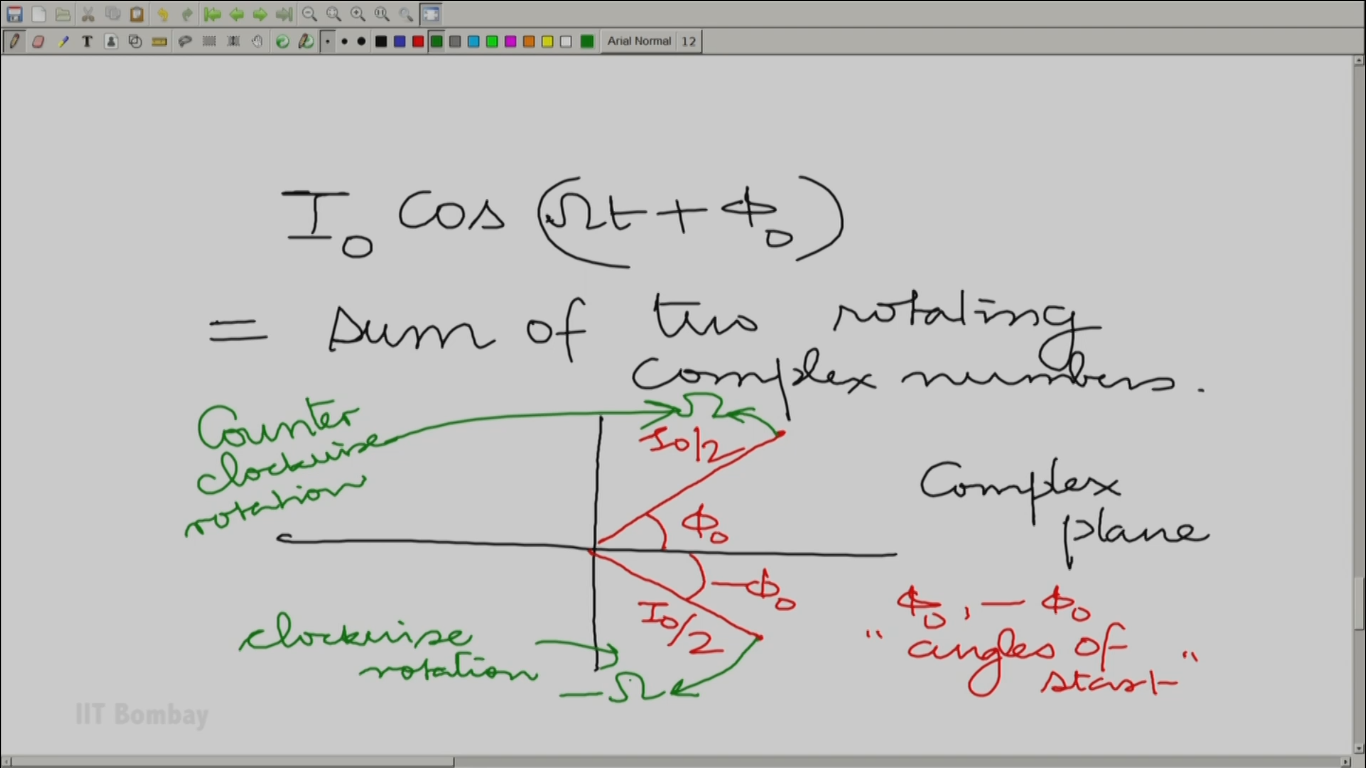
\includegraphics[scale=0.28]{rotating_complex.png}
\end{figure}
\\
We can express these two complex numbers in the polar form as
\[ c_1 = \frac{I_0}{2} e^{j \{ \Omega t + \phi_0 \}} \]
\[ c_2 = \frac{I_0}{2} e^{- j \{ \Omega t + \phi_0 \}} \]
where $j = \sqrt{- 1}$. One can see that $c_1 + c_2$ gives back the original
sinusoid.\\
It seems like a silly thing to do to describe a sinusoid as a combination of
two rotating complex numbers. But the reason for doing this is clear when we
look at the inductor once again.\\
Let's assume for now that we provide to the inductor, an input which is just
one of those rotating complex numbers. So
\[ I = \frac{I_0}{2} e^{j \{ \Omega t + \phi_0 \}} \]
Now, the voltage across an inductor is given by
\[ V = L \frac{d I}{d t} = L\frac{I_0}{2} (j \Omega) e^{j \{ \Omega t +
   \phi_0 \}} \]
Hence we can see that
\[ V / I = j \Omega L \]
Now the ratio of the voltage and current for an inductor is a complex
\textit{constant independent of time}!\\
Similarly, for the other rotating complex number, we will get $V / I$ again to
be a constant, but with a minus sign $(- j \Omega L)$. So in some sense the
actual angular frequency, whether positive or negative, is reflected. It is left as an exercise to do a similar analysis for capacitances and verify that
for capacitors,
\[ V / I = \frac{1}{j \Omega C} \]
This makes the analysis of RLC circuits (circuits consisting of Resistor(s),
Inductor(s) and Capacitors(s)) much easier as we can interpret these constants
as generalised resistances, or \textit{impedances.} In that sense, the
resistor has an impedance of $R$, an inductor has an inductance of $j \Omega
L$ and a capacitor has an impedance of $1 / j \Omega C$.\\
Notice that $c_1$ and $c_2$ defined above are complex conjugates of each
other. So whatever happens to $c_1$ is mirrored in $c_2$. For example, the $V
/ I$ for $c_2$ ($- j \Omega L$) is the complex conjugate of the $V / I$ for
$c_1$ ($j \Omega L$).\\
The analysis of sinusoids using rotating complex numbers is known as `phasor'
analysis. As the rotating complex numbers are constant in magnitude, but
change their phase, they are called `phasors'.\\
This is the reason why we earlier demanded that our systems should accept a
complex signal in general.\\
In a nutshell, dealing with amplitudes is easy but the dealing with phases is
a problem in sinusoids and that problem is overcame when you go to the phasor
instead of the corresponding sinusoid. Let us see how a general LSI system responds to
a phasor or sinusoid as an input.
\section{Module 2: Lecture 2\\Sinusoidal Input to LSI Systems}


%\subsection{Introduction}

\subsection{Understanding Phase Change In Sinusoids and Phasors}
We write a sinusoid as a combination of two rotating complex numbers, which we will henceforth call phasors, moving in opposite directions. 
\[
	2Acos(\Omega t + \phi) = Ae^{j(\Omega t + \phi)} + Ae^{-j(\Omega t + \phi)}
\]
Let us focus our attention on one of the phasors for now. Let us look at what happens when we introduce a phase change.\\
\[
Ae^{j(\Omega t + \phi)} \xrightarrow{Phase \ Change} Ae^{j(\Omega t + \phi + \Delta\phi)}
\]
\[
Ae^{j(\Omega t + \phi + \Delta\phi)} =
Ae^{j(\Omega t + \phi)}e^{j\Delta\phi}
\]
We hence find that a change of phase results just in a multiplying factor which is a constant independent of time.\\
Now we try to do a similar calculation for the complex conjugate (the phasor moving in the opposite direction).
\[
Ae^{-j(\Omega t + \phi)} \xrightarrow{Phase \ Change} Ae^{-j(\Omega t + \phi)}e^{-j\Delta\phi}
\]
Notice that the multiplying constant in this case is the complex conjugate of the previous multiplying factor we found.\\
\[
	2Acos(\Omega t + \phi) \xrightarrow{Phase \ Change} Ae^{j(\Omega t + \phi)}e^{j\Delta\phi} + Ae^{-j(\Omega t + \phi)}e^{-j\Delta\phi}
\]
We hence understand that using only one phasor is enough to fully determine the behaviour of the sinusoid. This explains why we used complex signals in our previous analysis, due to their ease in mathematical manipulation.\\
We will now see the result of inputting a sinusoidal signal to a stable linear shift invariant system, with impulse response $h(t)$ (Assume that the impulse response is real). We deal with stable LSI systems because the output will be bounded.\\
\begin{figure}[ht]
\begin{center}
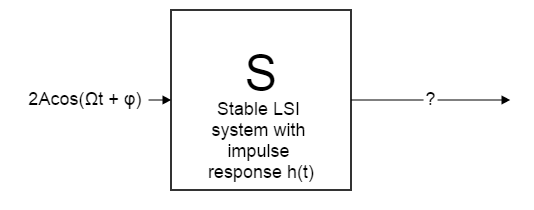
\includegraphics[width=10cm]{LSIcos.png}
\caption{Sinusoidal Input To Stable LSI System}
\end{center}
\end{figure}
The output for an LSI system is given by the convolution of the input and the impulse response.
The direct solution via convolution seems very difficult. In fact if we try to calculate the convolution integral, we get the following expression:
\[
y(t) = \int_{-\infty}^{+\infty} \! {h(\lambda)2Acos(\Omega(t-\lambda) + \phi) \ \dm \lambda}\]
We will now see how to solve it using phasors, making the analysis mathematically convenient.
%%%
%%%
\subsection{Phasor Input to LSI System}
Consider the output when a phasor is input to a stable LSI system.
\[
Ae^{j(\Omega t + \phi)} \xrightarrow{LSI} 
 \int_{\infty}^{\infty} \! Ae^{j(\Omega (t - \lambda) + \phi)}h(\lambda) \ \dm \lambda
\]
 
\[ =
Ae^{j(\Omega t + \phi)} \int_{\infty}^{\infty} \! {e^{-j\Omega\lambda}h(\lambda) \ \dm \lambda}
\]
Here, we see that we get the output to be the input phasor with a multiplying factor $\int_{-\infty}^{\infty} \! {e^{-j\Omega\lambda}h(\lambda) \ \dm \lambda}$, which is dependent only on $\Omega$ and $h$ (it is constant with respect to time).\\
We will now come back to the importance of why we chose our system to be stable. We will do this by trying to find a bound to the absolute value of the multiplying factor we just found.
\[
| \int_{-\infty}^{\infty} \! {e^{-j\Omega\lambda}h(\lambda) \ \dm \lambda} | \leq 
\int_{-\infty}^{\infty} \! { |e^{-j\Omega\lambda}||h(\lambda)| \ \dm \lambda }
\]
\[
\int_{-\infty}^{\infty} \! { |e^{-j\Omega\lambda}||h(\lambda)| \ \dm \lambda } =
\int_{-\infty}^{\infty} \! {|h(\lambda)| \ \dm \lambda }
\]
And as per the condition of stability the integral of the absolute value of the impulse response is bounded. Hence the absolute value of the multiplying factor is also bounded. In fact we have obtained a concrete bound to this integral, namely the absolute integral of the impulse response. We can do similar mathematical analysis for the conjugate as well.\\
This multiplying factor is called the \textit{Frequency Response} of the LSI system at angular frequency $\Omega$.
\[
	Frequency\ Response\ H(\Omega) = \int_{-\infty}^{\infty} \! {e^{-j\Omega\lambda}h(\lambda) \ \dm \lambda}
\] 
%%%
%%%
\subsection{Sinusoid Input to LSI System}
We will now come back to our original problem of inputting a sinusoidal signal into a stable linear shift invariant system. We will begin by simplifying the outputs of the two phasors.
\[
	H(\Omega)Ae^{j(\Omega t + \phi)} = |H(\Omega)|Ae^{j(\Omega t + \phi +  \angle  H(\Omega))}
\]
The complex conjugate of the frequency response is given by
\[
\bar{H}(\Omega) = \int_{-\infty}^{\infty} \! {e^{j\Omega\lambda}h(\lambda) \ \dm \lambda} = H(-\Omega)
\]
Note that the first equality holds only if $h(\lambda)$ is real.
Hence,
\[
H(-\Omega)Ae^{-j(\Omega t + \phi)} = |H(\Omega)|Ae^{-j(\Omega t + \phi +  \angle  H(\Omega))}
\]
So we can check by adding the two outputs that the output for inputting a sinusoid $2Acos(\Omega t + \phi)$ is given by:

\[
2Acos(\Omega t + \phi) \xrightarrow{Stable\ LSI} 2A|H(\Omega)|cos(\Omega t + \phi + \angle H(\Omega))
\]
This indicates that on passing through a stable LSI system, a sinusoid goes through an amplitude and phase shift which is independent of time and only dependent on the impulse response and angular frequency of the sinusoid. Note again that the impulse response has to be real for this to hold true.\\
Also, if we view an input to a stable LSI system as the sum of multiple sinusoids, the output can be visualized as the sum of the corresponding outputs of the sinusoids through the stable LSI system. The stability of the LSI systems guarantees the existence of the frequency response of the system. But if it is unstable it may or may not have a frequency response.
%%%
%%%
\subsection{Periodic Input to Shift Invariant Systems}
How does an LSI system respond to a general periodic signal? Consider the following lemma.\\
\textbf{Lemma:} A periodic input to a shift invariant system produces a periodic output.\\
\textbf{Proof:}\\
%%%
Let the input be $x(t)$ with a period $T$
\[x(t+T) = x(t)\ \ \forall t\]
\[x(t) \xrightarrow{SI\ system} y(t) \]
%%%
Now, by shift invariance,
\[x(t+T) \xrightarrow{SI\ system} y(t+T) \]
Hence,
\begin{equation}\label{eqn:PeriodicOutput}
y(t) = y(t+T)\ \ \forall \ t
\end{equation}
Hence the output is also periodic, infact with the same period $T$.\\
An important property of a periodic input or a periodic function is that it can be represented by a linear combination (which can be countably infinite) of sinusoids having frequencies which are multiples of the frequency of the input. This property is referred to as the existence of a Fourier Series expansion of the input. \\
The Fourier Series expansion and our understanding from the previous section gives us a simple method to compute the output of a periodic input in an LSI system as the linear combination of the output of these sinusoids.\\
%% Added paragraph for better flow. Needs verification:
This result, combined with \ref{eqn:PeriodicOutput} can be used to calculate the output for a general periodic input, but for that, we need still more information. How do we know whether a certain periodic signal can be expressed as a linear combination of sinusoids \emph{uniquely}? To answer this question, we need to invoke some concepts from linear algebra by considering signals as vectors.

%\subsection{Conclusion}
%In this lecture we understood the analysis of inputting sinusoidal input to a stable LSI system. We saw how we could simplify our analysis by the use of phasors. In the upcoming lecture we will learn about the use of inner product and vector analysis in understanding signals.


\section{Module 2: Lecture 3\\Signals and Vectors}

\subsection{Introduction}
In the previous lecture, we have learnt how a periodic input given to a Linear Shift Invariant system results in a periodic output with the same period. Now in this lecture we will see some new concepts by which every input can be expressed as sinusoidal inputs. Henceforth, it will be simpler to analyse their outputs.

\subsection{Relations between Signals and Vectors}
\label{sec:examples}
Consider a 2-dimensional vector, we can decompose this vector into two perpendicular components with $e_1$ and $e_2$ as the unit vectors along those directions. To find these components, we need to use Dot Product.
\subsubsection{Dot Product}
	Dot Product of two vectors u and v is defined as the magnitude of vector u multiplied by the magnitude of v multiplied by cosine of the angle between these two vectors.
    
	    					\begin{equation*}u.v = |u||v|cos\theta\end{equation*}
                            
where $\theta$ is the angle between vectors u and v. If u is a unit vector, then the dot product of vectors v and u gives the component of vector v in the direction of u, with the value |v|cos$\theta$.
	\begin{figure}[ht]
\centering
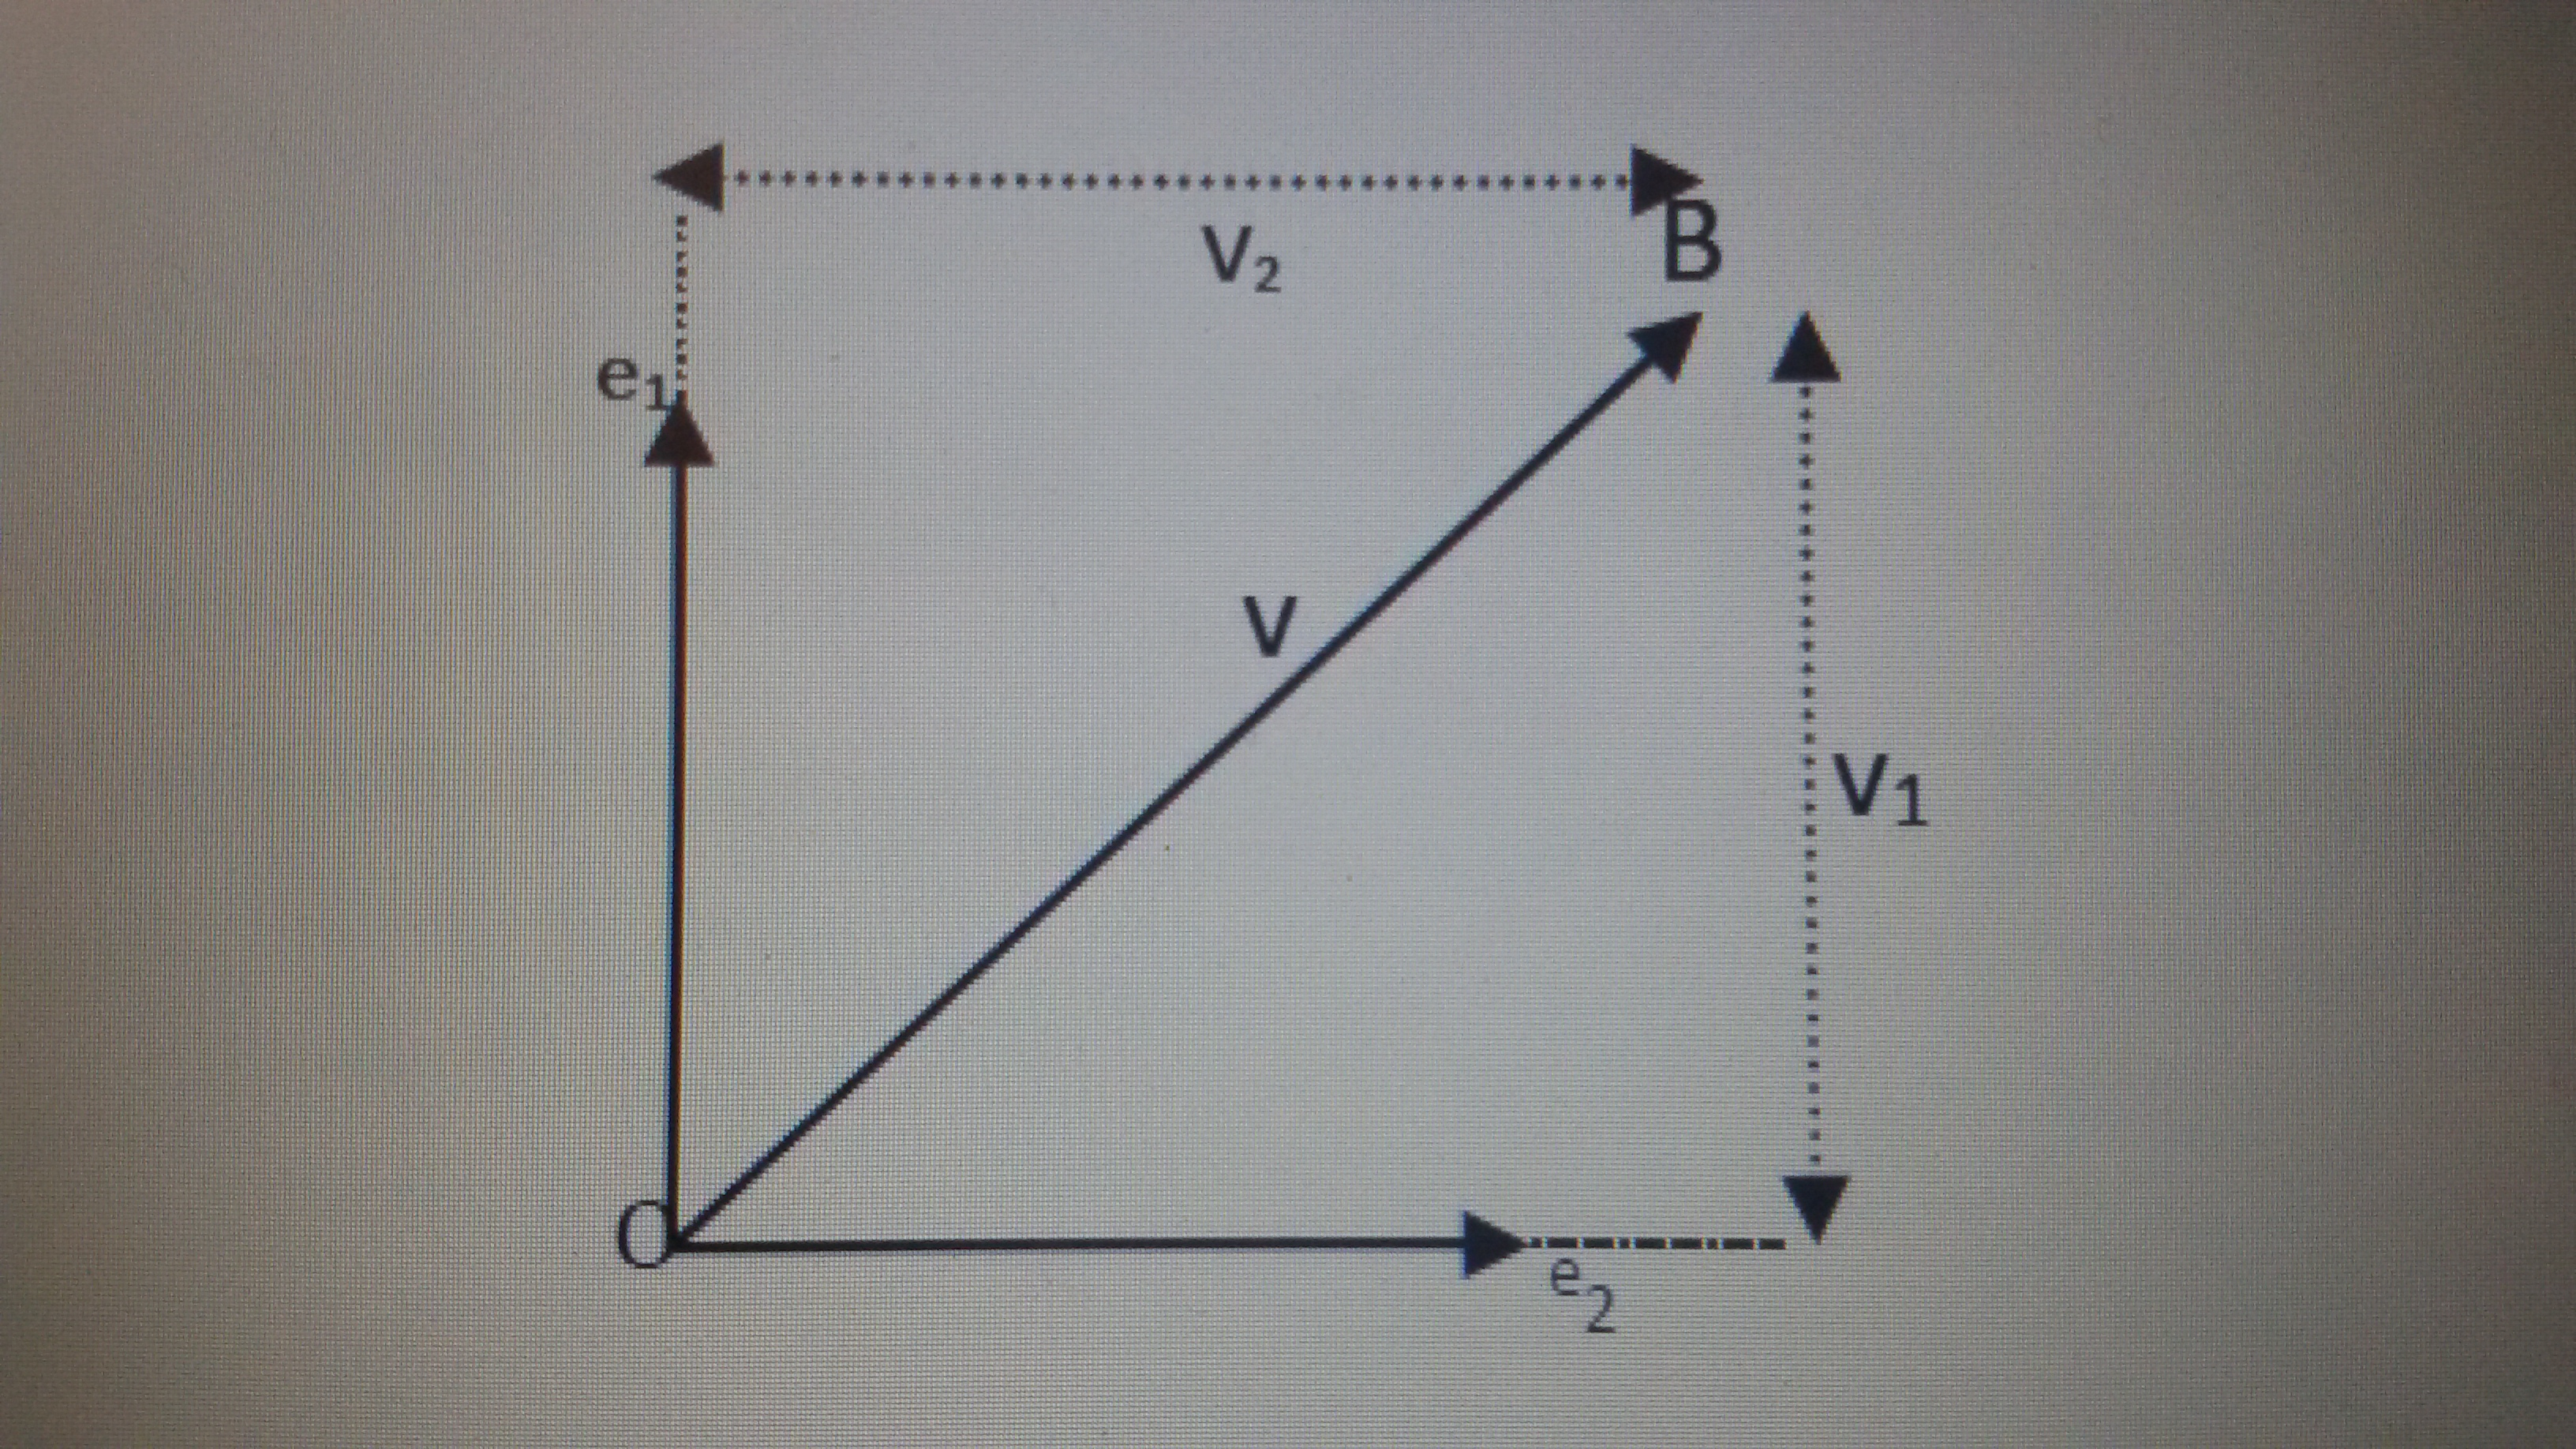
\includegraphics[scale=0.08]{figure.jpg}
\end{figure}
    
    
    Consider the above figure, here OB is a vector denoted by v which is expressed as
    \begin{equation*}v = v_1e_1 + v_2e_2\end{equation*}
    
    where $v_1$ and $v_2$ are the components in $e_1$ and $e_2$ directions respectively.
By this we can say that vectors $e_1$ and $e_2$ spans the space in 2D i.e. we can express any vector as a linear combination of e1 and e2. A collection of vectors span a space. Suppose if any vector can be expressed uniquely as a linear combination of $\{ u_1$,$u_2$,$u_3$ .... $u_n \}$, where $\{ u_1$,$u_2$,$u_3$...$u_n \}$ are linearly independent, then $\{ u_1$,$u_2$...$u_n \}$ is said to form a basis.\\
\noindent
Also, if $\langle u_i$,$u_j \rangle$ = 0 for i,j belonging from 1 to n,i.e. dot product of any two vectors is zero,  then the basis is said to be an \textit{orthogonal basis}. Finally, for a n-dimensional space, a collection of n linearly independent vectors forms the basis.\\
\noindent
The dot product of two vectors $u$ and $v$ is equal to the sum of the products of the corresponding perpendicular components. Suppose

				\begin{equation*}u = u_1e_1 + u_2e_2\end{equation*}
                        
                        \begin{equation*}v = v_1e_1 + v_2e_2\end{equation*} 
\noindent                        
                        therefore,\begin{equation*} u.v = u_1v_1 + u_2v_2\end{equation*}
           
\subsubsection{Dot Product of Discrete Sequences}           
Now, consider a discrete sequence with 2 non-zero points. This sequence can be compared to a 2-dimensional vector v with $v_1$ and $v_2$ as its perpendicular components such that it is equal to the values at the 2 non zero points of the sequence. Similarly for a sequence with n non-zero points can be considered as a vector in n dimensional space. Also, the concept of dot product is similarly applied to the discrete sequences.

For example : Consider
	x[n] = $(1/2)^n$ u[n];
    
    i.e.
     \begin{equation*}
    x[n] = (1/2)^n	\enspace	\enspace for\enspace	 n\geq0\end{equation*}
    \begin{equation*}	 0	\enspace  \enspace	 for\enspace	 n<0\end{equation*}
               
	 \begin{equation*} y[n] = (1/3)^nu[n] \end{equation*}
    
    i.e. 
    \begin{equation*}y[n] = (1/3)^n	\enspace \enspace	for\enspace n\geq0\end{equation*} \begin{equation*}0\enspace \enspace			for\enspace n<0 \end{equation*}
                  
                  
  Lets calculate the dot product of x[n] and y[n],i.e. summing the product of corresponding components.
  We have,
   \begin{equation*} \langle x[n],y[n] \rangle = \sum_{n=-\infty}^{\infty}\ x[n]y[n]\end{equation*} 
   \begin{equation*} \langle x[n],y[n] \rangle = \sum_{n=0}^{\infty}\ x[n]y[n]\end{equation*} 
   \begin{equation*} \langle x[n],y[n] \rangle = \sum_{n=0}^{\infty}\ (1/2)^n*(1/3)^n\end{equation*} 
   \begin{equation*} \langle x[n],y[n] \rangle = \sum_{n=0}^{\infty}\ (1/6)^n\end{equation*} 
   \begin{equation*} \langle x[n],y[n] \rangle = \frac{1}{(1-(1/6))}\end{equation*} 
   \begin{equation*} \langle x[n],y[n] \rangle = \frac{6}{5}\end{equation*} 
  		
          
 	By this we compute the dot product of two discrete sequences. This dot product is also called as \textit{Inner Product}. Inner product of two vectors $u$ and $v$ is represented by $\langle u,v \rangle$.

\subsubsection{Inner Product of Continuous Signals}
       In a discrete sequence, a unit vector can be expressed as $\delta[n-N]$ for all integers Z. A n-dimensional vector v can be expressed as
        \begin{equation*}v = v_1e_1 + v_2e_2 + ........ + v_ne_n\end{equation*}
        Now writing the above equation in terms of sequences, we have
       
    	\begin{equation*}	x[n] = 	\sum_{n=-\infty}^{\infty}\ x[N]\delta[n-N]\end{equation*}
            
            where x[n] is the component along dimension N.
       
Similarly applying the same concept for continuous time functions, we need to replace summation by integral, which gives,

					\begin{equation*}x(t) = \int_{-\infty}^{\infty} \! x(\lambda)\delta[t-\lambda] \ \mathrm{d}\lambda\end{equation*}
                    
             where x($\lambda$) is the component in direction $\lambda$ and $\delta[t-\lambda]$ is continuous impulse at $\lambda$ similar to unit vector.So inner product of x(t) and y(t) is given by
             
           \begin{equation*} \langle x(t),y(t) \rangle = \int_{-\infty}^{\infty} \! x(t)y(t) \ \mathrm{d} t\end{equation*}
             
 \subsection{Sinusoids with same period}
          Let us see how we can express any signal as sinusoidal functions. So, first we need to find sinusoidal signals which are perpendicular. Consider a signal x(t) which is periodic with period T,i.e. \begin{equation*}  x(t) = x(t+T)\end{equation*}. Assume that it can be expressed as a sum of sinusoidal functions. We should take a sinusoidal function which is periodic with period T. So it is of the form $A_k\cos (\frac{2\pi}{T}kt + \phi_k)$. We have,
          
          \begin{equation*}x(t) = \sum_{k=-\infty}^{\infty}\ A_k\cos (\frac{2\pi}{T}kt + \phi_k)\end{equation*}
          
          Let's take two different \textit{k}
.  \begin{equation*}
x_1 (t) = A_1 \cos (\frac{2\pi}{T}k_1t + \phi_1)
\end{equation*}
           and \begin{equation*}
x_2 (t) = A_2 \cos (\frac{2\pi}{T}k_2t + \phi_2)
\end{equation*}
          Consider the inner product of $x_1(t)$ and $x_2(t)$ with the interval going from 0 to T. We are here restricting our interval to T because the integral might diverge when we integrate from 0 to $\infty$. We have,
           \begin{equation*}\langle x_1(t),x_2(t) \rangle = \int_{0}^{T} \! x_1(t)x_2(t) \ \mathrm{d}t\end{equation*}
           \begin{equation*}\langle x_1 (t),x_2 (t) \rangle = \int_{0}^{T} \! \cos (\frac{2\pi}{T}k_1t + \phi_1) \cos (\frac{2\pi}{T}k_2t + \phi_2) \ \mathrm{d}t\end{equation*}
           Using 
          \begin{equation*} 2cosAcosB = cos(\frac{A+B}{2}) + cos(\frac{A-B}{2})\end{equation*}
          We have,
          \begin{equation*}\langle x_1 (t),x_2 (t) \rangle = \int_{0}^{T} \! \left\lbrace \cos (\frac{2\pi}{T}\frac{(k_1+k_2)}{2}t + \frac{\phi_1+\phi_2}{2}) + \cos (\frac{2\pi}{T}\frac{(k_1-k_2)}{2}t + \frac{\phi_1-\phi_2}{2}) \right\rbrace \ \mathrm{d}t \end{equation*}
          
          
        
        
                
                If ($k_1$ + $k_2$) or ($k_1$ - $k_2$) are not zero, that means we have a finite number of cycles of the sinusoids, implying the integral is zero. However if $k_1$=$k_2$, the second integral becomes T times $\cos (\theta_1-\theta_2)$.
                Thus we have,
            \begin{equation*} \langle x_1 (t),x_2 (t) \rangle  \neq 0	\enspace \enspace		for \enspace k_1 = k_2\end{equation*}
            \begin{equation*} \langle x_1 (t),x_2 (t) \rangle = 0	\enspace \enspace		for \enspace k_1 \neq k_2\end{equation*}
                
                
                Hence, we have proved that two sinusoids with same time period are perpendicular if they don't have same angular frequency and vice-versa. Thus using this important concept, we will be able to write any signal as sum of sinusoidal signals and hence analysis of these signals will be simpler.


\chapter{the second chapter}
\section{Module 2: Lecture 4\\Decomposition of Signals}

\subsection{Introduction}
\noindent
 A fundamental idea in the study of signals is to represent signals in terms of linear combination of \textit{basis} signals. In the previous section, we have embarked on some important concepts, relating to the idea of representing signals as a linear combination of sinusoids.
 %In this lecture, we will be recapitulating those ideas.
We assumed that we wish to look either at periodic signals or signals over a finite interval $T$. Without loss of generality, let that interval be $(0,T)$. 

\noindent
We have assumed that such signals are signals spanned by  all sinusoids of angular frequency $\Omega = \frac{2\pi}{T}kt,k=0, \pm1, \pm2 ..$

\noindent
The typical periodic function, with period $T$ is of the form
\begin{equation*}
  x(t) = \sum_{k=-\infty}^{\infty} \! A_k\cos (\frac{2\pi}{T}kt + \phi_k)
\end{equation*}
where $A_k$ denotes the amplitude, $\Omega = \frac{2\pi}{T}k$ is the angular frequency and $\phi_k$ the phase.
We had proved that these sinusoids are orthogonal if they don’t have same angular frequency.
\begin{equation*}
  \langle A_{k_1} \cos (\frac{2\pi}{T}k_1t + \phi_1),A_{k_2} \cos (\frac{2\pi}{T}k_2t + \phi_2)\rangle = 0 \enspace \enspace \text{for} \enspace k_1 \neq k_2 
\end{equation*}

\noindent
This important concept requires appreciating several different ideas. Using these ideas, we can decompose signal $x(t)$ in terms of sinusoids. However, there are some signals which can’t be spanned using these sinusoids. Such signals are beyond the scope of discussion that we are going to undertake at this stage.
%%%
%%%
\subsection{ Orthogonal vectors at a particular frequency}
\noindent
Consider a periodic signal $x(t)$ with fundamental period $T$. Then we can write $x(t)$ as
%Let us assume the signal $x(t)$ as
\begin{equation*}
  x(t) = \sum_{k=-\infty}^{\infty} \! A_k\cos (\frac{2\pi}{T}kt + \phi_k)
\end{equation*}
%where $x(t)$ is periodic with period $T$ and w
We constrain ourselves to $0<t<T$.

\noindent
To calculate $A_k$ and $\phi_k$ we need to use the following property i.e.
\begin{equation*}
\langle \cos (\frac{2\pi}{T}k_1t + \phi_1), \cos (\frac{2\pi}{T}k_2t + \phi_2) \rangle = 0 \enspace \enspace		for \enspace k_1 \neq k_2 \end{equation*}

\noindent
We can think of the cosines $\cos (\frac{2\pi}{T}kt + \phi_k)$ as countably infinite orthogonal vectors, indexed by $k$, for $k=0, \pm1, \pm2...$ and so on.

\noindent
To find out the component of $x(t)$ along these orthogonal vectors, we need to take the dot product of $x(t)$ with the unit vector, in the direction of orthogonal vectors $\cos(\frac{2\pi}{T}kt + \phi_k), 0<t<T$.
For calculating unit vector, we need to find the magnitude of the vector $\cos(\frac{2\pi}{T}kt + \phi_k)$ using dot product.

\begin{align*} \left|\cos(\frac{2\pi}{T}kt + \phi_k)\right| &= \langle \cos (\frac{2\pi}{T}kt + \phi_k), \cos (\frac{2\pi}{T}kt + \phi_k)\rangle \\
  &= \int_{0}^{T} \! \cos (\frac{2\pi}{T}kt + \phi_k) \cos (\frac{2\pi}{T}kt + \phi_k) \ \dm t \\
  &= \int_{0}^{T} \! \cos^2 (\frac{2\pi}{T}kt + \phi_k) \ \dm t \\
  &= \int_{0}^{T} \! (\frac{1}{2} + \cos (2(\frac{2\pi}{T}kt + \phi_k)) \ \dm t \\
  &= \int_{0}^{T} \! \frac{1}{2} \ \dm t + \int_{0}^{T} \! \cos (2(\frac{2\pi}{T}kt + \phi_k)) \ \dm t \\
  &= \frac{T}{2}
\end{align*}
%%%
Thus, the magnitude square of the cosine is $T/2$ and hence the magnitude is $\sqrt{T/2}$. So, the unit vector is given by

\begin{equation*} \textrm{Unit vector} = \sqrt{\frac{2}{T}}\cos (\frac{2\pi}{T}kt + \phi_k)\end{equation*}
                    
\noindent
But still, there is one unknown quantity, namely, $\phi_k$ in this unit vector. However, we can think of this vector as a vector in a two dimensional space:

\begin{equation*}\sqrt{\frac{2}{T}}\cos (\frac{2\pi}{T}kt + \phi_k) = \sqrt{\frac{2}{T}}[\cos\phi_k\cos (\frac{2\pi}{T}kt) - \sin\phi_k\sin (\frac{2\pi}{T}kt)] \end{equation*}
that is, the unit vector can be thought of as a linear combination of two vectors.

\noindent
We have,
\begin{align*}
  \langle \cos (\frac{2\pi}{T}kt + \phi_k), \sin (\frac{2\pi}{T}kt + \phi_k) \rangle &= \int_{0}^{T} \! \cos (\frac{2\pi}{T}kt + \phi_k) \sin (\frac{2\pi}{T}kt + \phi_k) \ \dm t  \\
  &= \frac{1}{2} \int_{0}^{T} \! 2 \cos (\frac{2\pi}{T}kt + \phi_k) \sin (\frac{2\pi}{T}kt + \phi_k) \ \dm t \\
  &= \frac{1}{2} \int_{0}^{T} \! \sin (\frac{4\pi}{T}kt + \phi_k) \ \dm t \\
  &= 0
\end{align*}
%%%
Hence, the cosine and sine components are also orthogonal. $\cos\phi_k$ and $\sin\phi_k$ are now two unknown constants.
%%%
Therefore, decomposing $x(t)$ along $\cos (\frac{2\pi}{T}kt + \phi_k)$ will give the same results as decomposing $x(t)$ along  $\cos (\frac{2\pi}{T}kt)$ and $\sin (\frac{2\pi}{T}kt)$. So, to decompose $x(t)$ along $\cos (\frac{2\pi}{T}kt)$ and $\sin (\frac{2\pi}{T}kt)$, we require unit vectors, which we already have calculated above.
%%%
So, the two unit vectors are $\sqrt{\frac{2}{T}}\cos (\frac{2\pi}{T}kt)$ and $\sqrt{\frac{2}{T}}\sin (\frac{2\pi}{T}kt)$.
%%%
%%% 
\subsection{Projection of Vectors}
Let $u_1$ = $\sqrt{\frac{2}{T}}\cos (\frac{2\pi}{T}kt)$ and $u_2 = \sqrt{\frac{2}{T}}\sin (\frac{2\pi}{T}kt)$. We know that at frequency $2\pi k/T$, there are two orthogonal vectors, $u_1$ and $u_2$. We have a two dimensional space and we need to calculate the component of the vector $x(t)$ along orthogonal vectors of this 2D space.
  
\noindent
 Let $v$ be any arbitrary vector of higher dimension and $v_p$ be the projection of $v$ onto our 2D space spanned by orthogonal vectors $u_1$ and $u_2$. To calculate the components of the vector $v$ along the two orthogonal vectors, we can project $v_p$  onto $u_1$ and $u_2$. We can also directly project $v$ onto $u_1$ and $u_2$.
 


\noindent
 The vector $v$ can be written as $v = v_p  + v_\perp$, where $v_p$ is the projection of $v$ on to 2D space and $v_\perp$ is component perpendicular to the 2D space . The projection of $v$ onto vectors $u_1$ and $u_2$ will be same as the projection of $v_p$  on those vectors, as the $v_\perp$ will not contribute in projection.
 
\begin{figure}[ht]
\centering
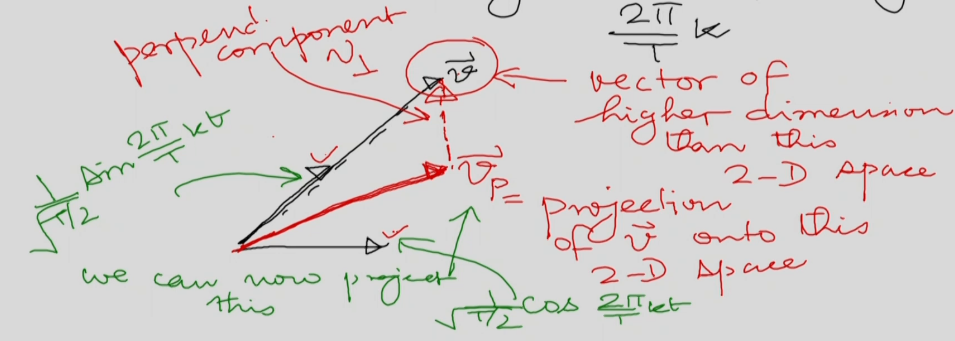
\includegraphics[scale=0.32]{S_215.PNG}		
\end{figure}

 \begin{figure}[ht]
\centering
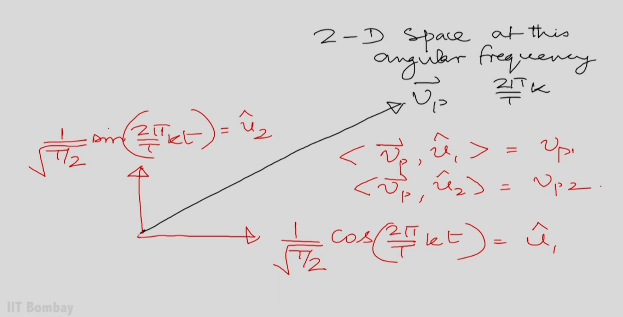
\includegraphics[scale=0.32]{S_215_2.PNG}		
\end{figure}

\noindent
Let us project $v_p$ along the two orthogonal vectors. 
  For projecting  $v_p$  along $u_1$ and $u_2$, taking dot product 
 
\begin{equation*} \langle v_p, u_1 \rangle =v_{p_1} \end{equation*}
\begin{equation*} \langle v_p, u_2 \rangle = v_{p_2} \end{equation*}
 
\noindent
$v_p$  in terms of $u_1$, $u_2$ can be written as $v_p$  = $v_{p_1}u_1$ + $v_{p_2}u_2$. Interestingly  $\langle v_p, u_1 \rangle = \langle v, u_1 \rangle$ is true also for $u_2$ as the perpendicular component $v_\perp$ is not going to contribute in the dot product. 
        
We know that the $k^{th}$ angular frequency =  $2 \pi k/T$.
At this frequency we have two components 
\begin{equation*}x(t) = \langle x(t), \sqrt{\frac{2}{T}}\cos (\frac{2\pi}{T}kt)\rangle \cdot \sqrt{\frac{2}{T}}\cos (\frac{2\pi}{T}kt) + \langle x(t), \sqrt{\frac{2}{T}}\sin (\frac{2\pi}{T}kt)\rangle \cdot \sqrt{\frac{2}{T}}\sin (\frac{2\pi}{T}kt)\end{equation*}
This can be simplified as

\begin{equation*}x(t) = \langle x(t), \cos (\frac{2\pi}{T}kt)\rangle \cdot \frac{2}{T}\cos (\frac{2\pi}{T}kt) + \langle x(t), \sin (\frac{2\pi}{T}kt)\rangle \cdot \frac{2}{T}\sin (\frac{2\pi}{T}kt)\end{equation*}

\noindent
\subsection{Decomposition of square wave}
We have a periodic signal $x(t)$ in Fig.\ref{fig:square-wave}, defined as
\[
x(t) =
\left\{
	\begin{array}{ll}
		1  & \mbox{if } 0 < t < \frac{T}{2} \\
		-1 & \mbox{if } \frac{T}{2} < t < T
	\end{array}
\right.
 \]

\noindent
$x(t) = x(t+T)$ for all $t$, i.e. $x(t)$ is periodic with period $T$.
              
\begin{figure}[ht]\label{fig:square-wave}
\centering
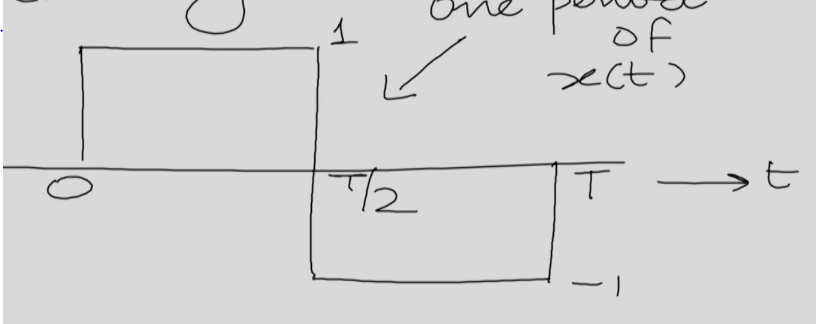
\includegraphics[scale=0.32]{S_216_1.PNG} %\\Figure 1
\caption{Plot of $x(t)$}
\end{figure}




\noindent
The zero frequency component is the  mean of $x(t)$ over a period $T$ which is $0$ since the net area under $x(t)$ in one period is zero.

\noindent
Let us calculate the quantity $\langle x(t), \cos (\frac{2\pi}{T}kt)\rangle \cdot \frac{2}{T}\cos (\frac{2\pi}{T}kt))$,


\noindent
For $k=1$ and $k=2$, we can see from Fig.\ref{fig:square-dot-cosine} that, the positive portion gets annulled by the negative portion. Similar is the case for $k=3, 4...$ and so on. Hence $\langle x(t), \cos (\frac{2\pi}{T}kt)\rangle= 0$ for given $x(t)$.


\begin{figure}[ht]\label{fig:square-dot-cosine}
\centering
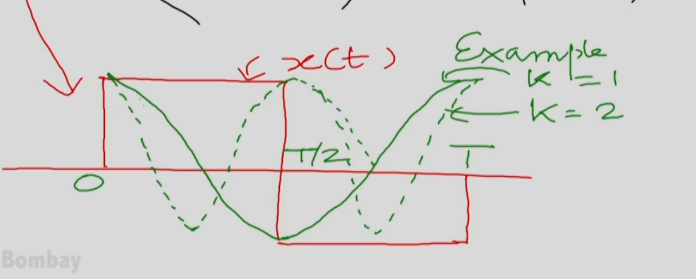
\includegraphics[scale=0.32]{s_216.PNG} %\\Figure 2
\caption{Dot product of the square wave with cosines}	
\end{figure}

\noindent
Calculating  $\langle x(t), \sin (\frac{2\pi}{T}kt)\rangle \cdot \frac{2}{T}\sin (\frac{2\pi}{T}kt)$, we have as shown in Fig.\ref{fig:square-dot-sine},

\begin{figure}[ht]\label{fig:square-dot-sine}
\centering
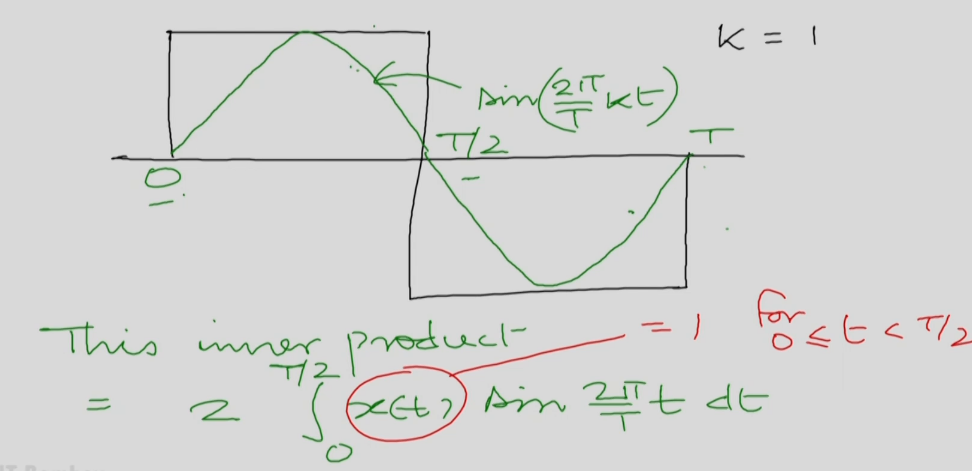
\includegraphics[scale=0.32]{S_216_3.PNG} %\\Figure 3
\caption{Dot product of the square wave with sines}	
\end{figure}
%%%
\begin{equation*} \langle x(t), \sin (\frac{2\pi}{T}kt)\rangle = \int_{0}^{T} \! x(t)\sin (\frac{2\pi}{T}kt) \ \dm t\end{equation*}
\begin{equation*} \langle x(t), \sin (\frac{2\pi}{T}kt)\rangle = \int_{0}^{\frac{T}{2}} \! \sin (\frac{2\pi}{T}kt) \ \dm t + \int_{\frac{T}{2}}^{T} \! {-\sin (\frac{2\pi}{T}kt)} \ \dm t \end{equation*}
\noindent
Also, we know that 
 \begin{equation*}\int_{0}^{\frac{T}{2}} \! \sin (\frac{2\pi}{T}kt) \ \dm t = -\int_{\frac{T}{2}}^{T} \! \sin (\frac{2\pi}{T}kt) \ \dm t \end{equation*}
\noindent
Using this, we have
\begin{equation*} \langle x(t), \sin (\frac{2\pi}{T}kt)\rangle = 2\int_{0}^{\frac{T}{2}} \! \sin (\frac{2\pi}{T}kt) \ \dm t = \left[-2\frac{\cos (\frac{2\pi}{T}kt)}{\frac{2\pi}{T}k}\right]_0^\frac{T}{2}\end{equation*}
%%%
For $k = 2n$, the above integral goes to zero as $\cos ({2\pi}n) = 1$ for all $n \in \mathbb{Z}$.
For $k = 2n-1$, the above integral has the value of $4T/\pi k$ because $\cos(2{\pi}(2n-1)) = -1$ for all $n \in \mathbb{Z}$. Thus,

\begin{equation*} \langle x(t), \sin (\frac{2\pi}{T}kt)\rangle = \frac{4T}{{\pi}k} \textrm{ (for odd }k) \end{equation*}
\noindent
Hence, we have, after multiplying by $2/T$,
\begin{equation*} x(t) = \sum_{n=1}^{\infty}\ \frac{4}{{\pi}(2k-1)} \sin (\frac{2\pi}{T}(2k-1)t)\end{equation*} 

\subsection{Examples of Decomposition}
\subsubsection{Exercise 1} 
\noindent
Work out the decomposition for an asymmetric square wave, of period $T$ as shown in the figure below.
\begin{figure}[ht]
\centering
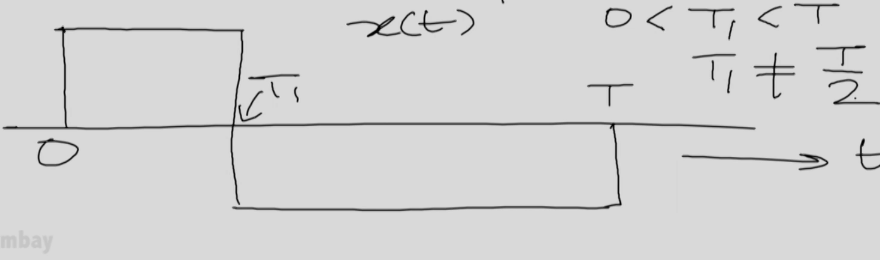
\includegraphics[scale=0.32]{S_217_1.PNG}
\end{figure}
 				\begin{equation*} x(t) = 1 \enspace \enspace      0<t<T_1 \end{equation*}
       			\begin{equation*} x(t) = -1  \enspace\enspace 	T_1 < t< T \end{equation*} \begin{equation*}0<T_1<T, \enspace T1\neq T/2, x(t+T) = x(t)\enspace  \forall t\in R.  \end{equation*}

                
\subsubsection{Exercise 2}
\noindent
In the answer of exercise 1 put $T_1 =T/2$, and verify the answer with that of decomposition of symmetric square wave.

\subsubsection{Exercise 3}
\noindent
Work out the decomposition for symmetric triangular wave, periodic with period $T$.

\noindent
\textit{Hint}: Use and observe the symmetry graphically.
\begin{figure}[ht]
\centering
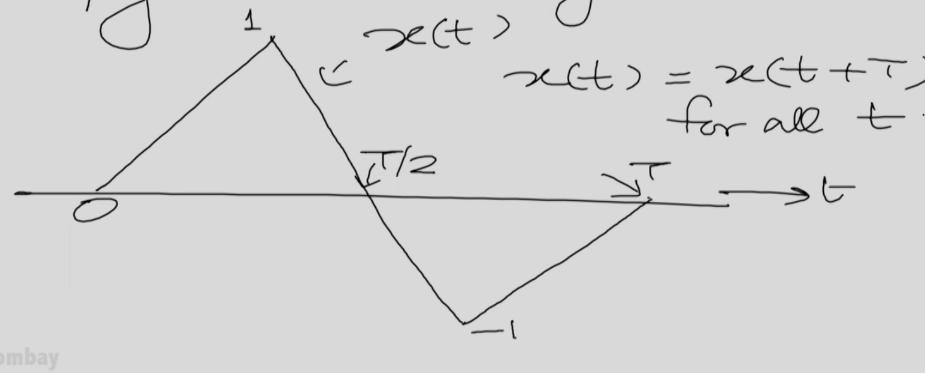
\includegraphics[scale=0.32]{S_217_2.PNG}
\end{figure}


\subsubsection{Exercise 4}
\noindent
Evaluate the decomposition for an asymmetric triangular wave as shown in the figure. Cross check the answer with that of exercise 3, by putting  $T_1 = T/2$ in the final answer.
\begin{figure}[ht]
\centering
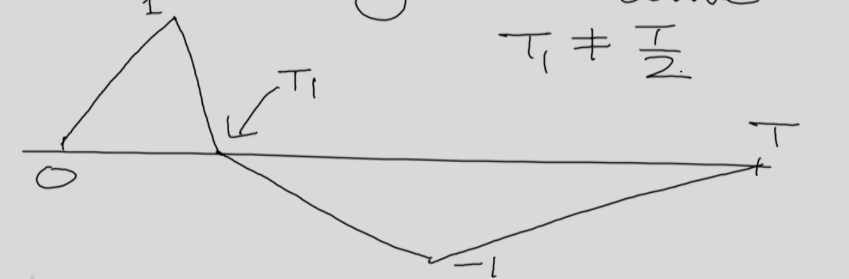
\includegraphics[scale=0.32]{S_217_3.PNG}
\end{figure}


\subsubsection{Exercise 5}
\noindent
A variant of symmetric triangular wave is shown below. Find its decomposition and compare with answer of exercise 3.
\begin{figure}[ht]
\centering
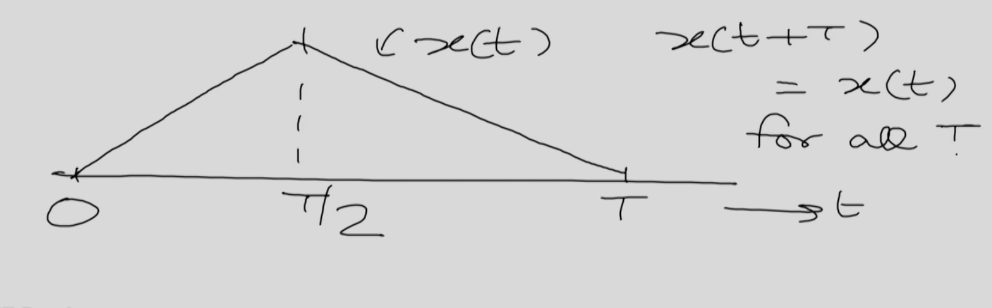
\includegraphics[scale=0.32]{S_217_4.PNG}
\end{figure}

\pagebreak

\subsubsection{Exercise 6}
\noindent
A variant of an asymmetric triangular wave is shown below. Evaluate the decomposition of  this wave. Substitute $T_1 = T/2$, in the answer and compare with the result of exercise 5. Explain the differences in the result, if any.
\begin{figure}[ht]
\centering
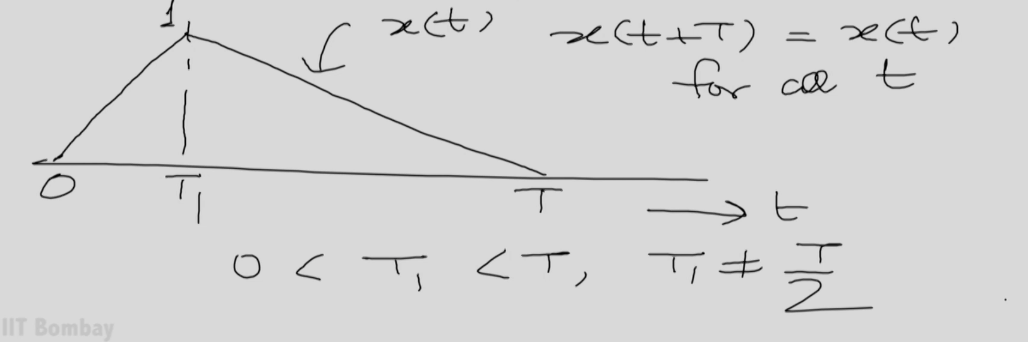
\includegraphics[scale=0.32]{S_217_5.PNG}
\end{figure}








                



                     

\section{Module 2: Lecture 5\\Fourier Series Decomposition and its Applications}

\subsection{Introduction}
We have been decomposing periodic waveform into their periodic sinusoidal components. In this lecture we look at a variation of the same decomposition using complex exponential functions. One way of doing this is to convert each sinusoidal component of sinusoidal decomposition into corresponding exponential functions. However, in some cases, we prefer to a priori decompose the waveform in complex exponential components.
\newline
We shall also see how to go from the complex exponential components to sinusoidal components. We will then look at the applications of both sinusoidal and complex exponential decompositions; in particular, we will be analyzing its utility in determining the output from a linear shift invariant system on applying a periodic input.
We will also see some conditions under which we cannot obtain a Fourier series decomposition for a periodic waveform.

\subsection{Complex Exponential Fourier Series Decomposition}
Suppose we are given a periodic signal $x(t)$ with period $T$. We wish to write $x(t)$ in terms of sum of complex exponential functions:
$$ x(t) = \sum_{k=-\infty}^{\infty}{C_{k} \ e^{j2\pi kt/T}} $$
where $C_k$ belongs to the set of complex numbers.
Basically, we are trying to write $x(t)$ as a linear combination complex exponential functions rotating at angular frequencies $2\pi k/T$ for all integer $k$. Notice that complex exponentials with angular frequencies as positive integral multiples of $2\pi kt/T$ represent anticlockwise rotating phasors while the complex exponentials with negative angular frequencies represent clockwise rotating phasors.
\newline
\subsubsection{Orthogonality of Fourier Series Components}
We now establish orthogonality between the complex exponential components.
We take 2 integers $k$ and $l$ and evaluate the inner product
\begin{equation}
\int_{-T/2}^{T/2}{\frac{1}{T}e^{(j2\pi kt/T)}e^{(j2\pi (-l)t/T)}}dt = \int_{-T/2}^{T/2}{\frac{1}{T}e^{(j2\pi (k-l)t/T)}}dt
\end{equation}
We have 2 cases now:
\begin{itemize}
\item {\textbf{Case 1}} $k=l$ The integral in (1) becomes $\int_{-T/2}^{T/2}\frac{1}{T}dt = 1$
\item {\textbf{Case 2}} $k \neq l$ The integral in (1) becomes $$\int_{-T/2}^{T/2}{\frac{1}{T}e^{(j2\pi (k-l)t/T)}}dt = \frac{1}{T}\frac{e^{(j2\pi (k-l)t/T)}}{(j2\pi (k-l)/T)}\Bigg|_{-T/2}^{T/2} = 0$$
\end{itemize}
\subsubsection{Obtaining Complex exponential Decomposition from Sinusoidal Decomposition}
Suppose we are given the sinusoidal components of the decomposition of a real waveform $$x(t) = \sum_{0}^{\infty}A_{k}\cos(2\pi kt/T + \phi_{k})$$
Note that in the above sum, for $k = 0$, we will have the component as $A_{0}\cos(\phi_{0})$, we can merge constant $\cos(\phi_{0})$ into $A_{0}$ and we will simply have constant $A_{0}$ for $k = 0$.
Now for a non-zero integer $k$ using $\cos(\theta) = \frac{1}{2}(e^{j\theta} + (e^{j\theta})^{*})$, (Note: $C^{*}$ denotes complex conjugate of $C$), we have $$A_{k}\cos(2\pi kt/T + \phi_{k}) = \frac{1}{2}\Bigg(A_{k}e^{j\phi_{k}}e^{j2\pi kt/T} + (A_{k}e^{j\phi_{k}})^{*} (e^{-j2\pi kt/T})\Bigg)$$
since $A_k$ are real.
$$\implies C_{k} = \frac{1}{2}A_{k}e^{j\phi_{k}}$$
$$\implies C_{-k} = \frac{1}{2}(A_{k}e^{j\phi_{k}})^{*}$$
And we also have trivially $C_{0} = A_{0}$
Notice that for real waveform, we have $C_{k} = (C_{-k})^{*}$


\subsubsection{Converting Complex Exponential to Sinusoidal Decomposition}
Suppose we are given a real $$ x(t) = \sum_{k=1}^{\infty}{C_{k}e^{(j2\pi kt/T)}} + \sum_{k=-\infty}^{-1}{C_{k}e^{(j2\pi kt/T)}} + C_{0}$$
Now, note that for an integer $k \neq 0$, $$\int_{-T/2}^{T/2}e^{(j2\pi kt/T)}dt = \frac{1}{T}\frac{e^{(j2\pi kt/T)}}{(j2\pi k/T)}\Bigg|_{-T/2}^{T/2} = 0$$
whereas, for k = 0, $$\int_{-T/2}^{T/2}1dt = T$$
So, basically we can obtain $C_{0}$ by integrating $x(t)$ over time $T$. In the Fourier Decomposition only $C_{0}$ will give a non zero integral which is equal to $C_{0}\cdot T$
Hence, $$C_{0} = \frac{1}{T}\int_{-T/2}^{T/2}x(t)dt$$
Now, since for real $x(t)$ we have $C_{k} = (C_{-k})^{*}$, we get
$$C_{k}e^{j2\pi kt/T} = (C_{-k}e^{-j2\pi kt/T})^{*}$$ So we have $$C_{k}e^{j2\pi kt/T} + C_{-k}e^{-j2\pi kt/T} = 2 Re (C_{k}e^{j2\pi kt/T})$$
Using the polar form of $C_{k}$ which is $|{C_{k}}|e^\phi_{k}$, we get
$$ 2 Re (C_{k}e^{j2\pi kt/T}) =  2|{C_{k}}|Re(e^{j2\pi kt/T + \phi_{k}} = 2|{C_{k}}|\cos(j2\pi kt/T + \phi_{k})$$
Finally, we have the sinusoidal decomposition
$$x(t) = C_{0} + \sum_{k=1}^{\infty}2|{C_{k}}|\cos(j2\pi kt/T + \phi_{k})$$

\subsection{Periodic Input to a Simple RC Circuit}

Suppose, we apply a real periodic voltage waveform $x(t)$ as input to a series RC-circuit with time period $T$. Recall that an RC circuit is a linear shift invariant system. Suppose we can write complex exponential decomposition of $x(t)$ as $$\sum_{k=-\infty}^{\infty}{C_{k}e^{(j2\pi kt/T)}}$$ The advantage of doing this is that we can use the fact that a complex exponential input to a linear shift invariant system simply gives the same complex exponential multiplied by a constant as its ouput. By phasor analysis of the circuit, we have the transfer function $$ \frac{j(2\pi k/T) CR}{1 + j(2\pi k/T) CR}$$
So, the output waveform will be simply $$y(t) = \sum_{k=-\infty}^{\infty} \frac{j(2\pi k/T) CR}{1 + j(2\pi k/T) CR} {C_{k}e^{(j2\pi kt/T)}}$$


This illustrates the power of having complex exponential decomposition of a waveform since we can obtain the output waveform quite simply if it is passed through a linear shift invariant system. Now, one catch in the above discussion is that we assumed that the decomposition of $x(t)$ in to a Fourier series is possible. It turns out it's \emph{not} always the case that we can write a Fourier series decomposition for a periodic waveform! Although, for most of the practical waveforms, we can write it. We will look at the conditions under which we can write the Fourier series decomposition for a periodic waveform. There are some waveforms for which we cannot find the Fourier decomposition. One such example is $x(t) = \sin{(1/frac(t))}$ where $frac(t)$ denotes fractional part of $t$. So, $x(t)$ is periodic with period 1 but still its Fourier series decomposition fails to exist. There are certain conditions under which Fourier analysis can be done, they are called the ‘Dirichlet’ Conditions. We shall not discuss them here.


\subsection{Periodic Inputs to a General Linear Shift Invariant System}

In this section we use Fourier series decomposition to determine output from a linear shift invariant system on applying a periodic input waveform. Of course for our analysis, will assume that Fourier series decomposition of the input waveform exists.
\newline
Let $\mathbb{S}$ denote a linear shift invariant system, let $h(t)$ be its impulse response. We apply a periodic input waveform $x(t)$. Now, using linearity of the system, output of the system is simply the sum of output obtained for each component of Fourier series decomposition of $x(t)$.
\newline
Let us derive the output for the $k^{\textnormal{th}}$ component of $x(t)$. The output for $k^{\textnormal{th}}$ will be the convolution of $h(t)$ and the input itself 
	$$\int_{-\infty}^{\infty}{h(\tau) \cdot C_{k}e^{j2\pi k(t- \tau)/T}}d \tau$$ Since, the above integral runs over $\tau$ and not $t$, the above expression reduces to 
    $$C_{k}e^{j2\pi kt/T}\int_{-\infty}^{\infty}{h(\tau) \cdot e^{-j2\pi k\tau/T}} d \tau$$
The integral reduces to a constant depending on k. So, what we obtain is quite interesting as it is simply the input itself multiplied by a constant!
Let us denote the constant by $\mathcal{H}(k)$. So, the output which is the sum of the outputs obtained for each component is
$$\sum_{k=-\infty}^{\infty}\mathcal{H}(k)C_{k}e^{j2\pi kt/T}$$

\subsection {Conclusion} In this lecture we discussed about Fourier series decomposition, its properties and its application in analysing linear shift invariant systems. In the coming lectures, we will discuss the significance of the quantity $\mathcal{H}(k)$ we derived in previous section and begin with what is known as Fourier Transform.







\section{Module 2: Lecture 6\\The Fourier Transform}

\subsection{Introduction}
We are now in a position where we can deal with more general signals from the point of view of decomposition into sinusoidal frequency components and analysis as to what happens when you pass them through a linear shift invariant system. To do that, let's recapitulate some of the important conclusions that we had drawn in the previous chapter which will now help us in generalization.
%%%
%%%
\subsection{Recapitulation}
Let $\mathbb{S}$ be a linear shift invariant system with impulse response $h(t)$, and to it, we give a periodic signal input. Let’s assume that the Dirichlet conditions are obeyed. So we could decompose this into its Fourier series.
\begin{equation*}
x(t)= \sum\limits_{k=-\infty}^{k=+\infty}c(k)e^{j\Omega kt}
\end{equation*}
Where $\Omega=2\pi /T$ is the angular frequency and $c(k)$ are the Fourier coefficients. Now, the output can also be written as a Fourier series.
\begin{equation*}
y(t)= \sum\limits_{k=-\infty}^{k=+\infty}c(k)H(k\Omega)e^{j\Omega kt}
\end{equation*}
where
\begin{equation*}
H(\Omega)= \int_{-\infty}^{+\infty} \! h(t)e^{-j\Omega t} \ \dm t
\end{equation*}
%%%
%%%
\subsection{Interpretation of $H(\Omega)$ as a Dot Product}
We can interpret $H(\Omega)$ as a dot product or inner product. It’s an inner product between the impulse response $h(t)$ and the rotating phasor $e^{j\Omega t}$. An inner product with a unit vector calculates the projection or a component of the vector along the unit vector. So it's as if we are trying to find the component of the impulse response along a rotating phasor, rotating with an angular velocity $\Omega$. And, at the specific values of $\Omega$ given by each of the Fourier series components, we evaluate this dot product and use it to modify the Fourier series coefficient.
We can see from the equation of output $y(t)$ that output Fourier series coefficients are $c(k)H(\Omega k)$. Recall that in the input, the Fourier series coefficients were calculated by taking an inner product taking only one period of the input for the integral.
We took only one period of the input, and found the inner product with the corresponding harmonic or the complex exponential rotating with that particular multiple of the fundamental frequency. This is how we calculate the Fourier series coefficients.\\
Now, we can see that the Fourier coefficients of the output are the \emph{component by component multiplication of the Fourier coefficients of the input and impulse response}.
\[
Y(k\Omega)= c(k)H(k\Omega)
\]
Now, there are two questions to answer here. Here we have assumed that the input was periodic. What if it is not? Can we generalize this to a non-periodic function is a question that we need to answer. Secondly, can we think of this quantity $H(\Omega)$ as a new transform or a new way of dealing with the impulse response in its own right?\\
Now, a transform will make sense or will be adequate only if it is invertible. That is to say, we should be able to get back $h(t)$ from $H(\Omega)$. There should be no loss of information. It turns out that this is indeed the case. We can call $H(\Omega)$, for any $\Omega \in \mathbb{R}$, as the \emph{Fourier transform} of the impulse response $h(t)$.\\
Now let's try to address the question as to how can we \emph{go back} to $h(t)$ from $H(\Omega)$.
%%%
%%%
\subsection{Inverse for the Fourier Transform}
The answer to the question again lies in vector intuition. As we have seen, $H(\Omega)$ is the component of $h(t)$ along the phasor $e^{j\Omega t}$ for all such $\Omega \in \mathbb{R}$. In vector algebra, we get back a vector from its components by multiplying the components with their corresponding unit vectors and summing them. So, if $\hat{u}_1$ and $\hat{u}_2$ are two orthogonal unit vectors in two dimensions, $\overrightarrow{v}$ is a 2-D vector, and
\[
\langle \overrightarrow{v},\hat{u}_1 \rangle = v_1, \langle \overrightarrow{v},\hat{u}_2 \rangle = v_2
\]
Then, we construct $\overrightarrow{v}$ by multiplying the components with the corresponding unit vector and summing them. Hence
\[
\overrightarrow{v} = v_1\hat{u}_1 + v_2\hat{u}_2
\]
Now using the same principle here, $H(\Omega)$ are the components of the ``vector'' $h(t)$ along the unit vectors $e^{j\Omega t}$. Hence, to obtain the vector $h(t)$ back, we should multiply the component by the unit vector and sum up, or in this case, integrate over all $\Omega$.\\
But there are two subtleties involved here. Firstly, we don't know whether in this vector space of integrable functions, the vector $e^{j\Omega t}$ is a unit vector or not. That is, whether its magnitude is one or not. In case it is not one, we have to multiply it by a suitable constant to make it a unit vector. Secondly, we don't know whether $e^{j\Omega_1 t}$ and $e^{j\Omega_2 t}$ are orthogonal or not, for $\Omega_1 \neq \Omega_2$.\\
In the following subsection, we proceed to evaluate the inverse of $H(\Omega)$ assuming two things; one is that the vectors $e^{j\Omega t}$ are orthogonal, and that the multiplying factor $\kappa_0$ (for making it a unit vector) is independent of $\Omega$.
%%%
%%%
\subsubsection{Finding the Inverse of the Fourier Transform}
Form the previous discussion, the quantity we propose to be the inverse of $H(\Omega)$ is given by
\[
I = \int_{-\infty}^{\infty} \! H(\Omega)\ \kappa_0 e^{j\Omega t} \ \dm \Omega
\]
Now, we know that
\[
H(\Omega)= \int_{-\infty}^{\infty} \! h(t_1)e^{-j\Omega t_1} \ \dm t_1
\]
Putting this in $I$, we get,
\[
I = \int_{-\infty}^{\infty} \! \int_{-\infty}^{\infty} \! h(t_1)e^{-j\Omega t_1}\ \dm t_1 \ \kappa_0 e^{j\Omega t} \ \dm \Omega
\]
\[
= \int_{-\infty}^{\infty} \! h(t_1) \left\lbrace \int_{-\infty}^{\infty} \! \kappa_0 e^{-j\Omega t_1} \  e^{j\Omega t} \ \dm \Omega \right\rbrace \dm t_1
\]
Let's evaluate the quantity in the braces. We can write it as
\[
\lim_{\Omega_1 \to \infty} \int_{-\Omega_1}^{+\Omega_1} \! \kappa_0 e^{j\Omega (t-t_1)} \ \mathrm{d}\Omega
\]

\[
= \lim_{\Omega_1 \to \infty} \kappa_0 \frac{e^{j\Omega_1 (t-t_1)}-e^{-j\Omega (t-t_1)}}{j(t-t_1)}
\]

\[
= \lim_{\Omega_1 \to \infty}\frac{2\kappa_0 j\sin(\Omega_1 (t-t_1))}{j(t-t_1)}
\]

\[
= \lim_{\Omega_1 \to \infty}\frac{2\kappa_0\Omega_1\sin(\Omega_1 (t-t_1))}{\Omega_1(t-t_1)}
\]

Now, this can be written as 
\[
\lim_{\Omega_1 \to \infty} 2\kappa_0\Omega_1 \frac{\sin(x)}{x}
\]
where $x=\Omega_1(t-t_1)$. Now, $\sin(x)/x$ is not defined at $x=0$ as it has a zero divided by zero form. So we evaluate the limit as $x\to 0$.
\[
\lim_{x \to 0}\frac{\sin(x)}{x} = \lim_{x \to 0}\frac{\cos(x)}{1} = 1
\]
where the first equality is due to L'H\^opital's rule. This function will be oscillatory due to $\sin(x)$, but will decay as $x$ increases, due to the $x$ in the denominator. Also, the function will be zero when $x=n\pi$ or $\Omega_1(t-t_1)=n\pi$. Now, let's deal with this function as a function of $(t-t_1)$ rather than $x$. Let us try to plot the function
\[
f(t-t_1) = \frac{2\kappa_0\Omega_1\sin(\Omega_1 (t-t_1))}{\Omega_1(t-t_1)}
\]
The value of $\sin(x)/x$ is $1$ as $x \to 0$ as we saw earlier. Hence $f(0)=2\kappa_0\Omega_1$. Also the first null of the function will occur at $\Omega_1(t-t_1)=\pi$ or $(t-t_1)=\pi/\Omega_1$. Also the function is even with respect to $(t-t_1)$.
\begin{figure}[ht]
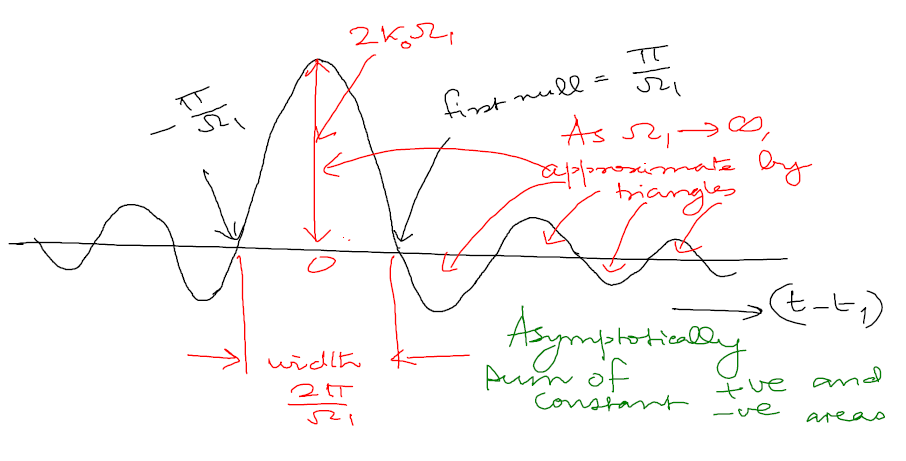
\includegraphics[scale=0.6]{fig.png}
\label{fig:sinc}
\caption{Sinc function}
\end{figure}
Hence, we will get a plot roughly as shown in Fig.\ref{fig:sinc}.
Now, we have to look at what happens when $\Omega_1 \to \infty$. We can see that the height of the main lobe at $x=0$ goes to infinity, but the width of the lobe, which is $2\pi/\Omega_1$ goes to zero, as $\Omega_1 \to \infty$. It can also be shown that the area of the other smaller lobes add up to zero, due to their alternating nature. Hence, we have a \emph{pulse} whose height is tending to infinity and the width to zero. In that case, we can assume the central lobe to be a triangle. Hence its area will be
\[
A = \frac{1}{2}\frac{2\pi}{\Omega_1}2\kappa_0\Omega_1 = 2\pi\kappa_0
\]
Hence, we can see that this area is a constant independent of $\Omega_1$. So we have a pulse having infinite magnitude and zero width, with a constant area encapsulated by it, and as you will remember from Part 1, this is nothing but the \emph{impulse function} $2\pi\kappa_0\delta(t-t_1)$.\\
Now, going back to our integral $I$,
\[
I = \int_{-\infty}^{\infty} \! h(t_1) \left\lbrace \int_{-\infty}^{+\infty} \! \kappa_0 e^{-j\Omega t_1} \  e^{j\Omega t} \ \mathrm{d}\Omega \right\rbrace \mathrm{d}t_1
\]
And we have evaluated the quantity in the braces to be $2\pi\kappa_0\delta(t-t_1)$. Hence,
\[
I = \int_{-\infty}^{\infty} \! h(t_1)\left\lbrace 2\pi\kappa_0\delta(t-t_1) \right\rbrace \mathrm{d}t_1 = 2\pi\kappa_0 \int_{-\infty}^{\infty} \! h(t_1) \delta(t-t_1)\ \mathrm{d}t_1
\]
Hence, by the sifting property of the delta function, we have,
\[
I = 2\pi\kappa_0 h(t)
\]
Hence, we can now set the value of $\kappa_0$ such that $I = h(t)$ as required. Hence $\kappa_0 = 1/2\pi$.\\
Hence, we finally have our expression for the \emph{Inverse Fourier transform} of $H(\Omega)$.
\[
h(t) = \frac{1}{2\pi}\int_{-\infty}^{\infty} \! H(\Omega)\  e^{j\Omega t} \ \mathrm{d}\Omega
\]
%%%
%%%
\subsection{Orthogonality of the Complex Exponentials}
A valid question to ask here is where did the orthogonality of the complex exponentials come in the picture. The answer lies in the integral in the braces which we evaluated.
\[
\int_{-\infty}^{+\infty} \! \kappa_0 e^{-j\Omega t_1} \  e^{j\Omega t} \ \mathrm{d}\Omega = 2\pi\kappa_0 \delta(t-t_1)
\]
or,
\[
\int_{-\infty}^{+\infty} \! e^{j\Omega t} \ \overline{e^{j\Omega t_1}} \ \mathrm{d}\Omega = 2\pi \delta(t-t_1)
\]
where the bar indicates complex conjugate. Now, this can be also written by renaming the variables, treating $t$ as the independent variable, as
\[
\int_{-\infty}^{+\infty} \! e^{j\Omega_1 t} \ \overline{e^{j\Omega_2 t}} \ \mathrm{d}t = 2\pi \delta(\Omega_1-\Omega_2)
\]
Now, we can immediately see that this is like an inner product between phasors rotating with different frequencies $\Omega_1$ and $\Omega_2$, and what this statement says is that it is non zero only for $\Omega_1=\Omega_2$. Hence, we do have some sense of orthogonality here. But since the value is infinite when the frequencies are equal, we have to call this a generalized orthogonality relation.
%%%
%%%
\subsection {Implications} 
Let's try to find what the Fourier transform expression implies. We have a non-periodic function $h(t)$ and we have decomposed it in its Fourier coefficients, not for discrete, but continuous set of frequency values, from minus to plus infinity. This can be thought of in the following way: We think of a non-periodic function as a periodic function with period tending to infinity. This is a valid statement, because as a periodic with period $T$ repeats itself after an interval $T$, we can say that a non-periodic function repeats itself after $T \to \infty$. Now, as the time period increases, the spacing between two adjacent frequencies decreases. And
\[
f = \lim_{T\to\infty}\frac{2\pi}{T} = 0.
\]
Hence, for a non-periodic function, the spacing between the adjacent frequencies tends to zero, which amounts to the Fourier spectrum going to continuous from discrete. This is exactly what has happened. The Fourier transform $H(\Omega)$ is a continuous function, and in general has a non-zero value for all $\Omega \in \mathbb{R}$.






\section{Module 2: Lecture 7\\Fourier Transforms properties and Fourier series example}

\subsection{Introduction}
	In this section, we will take a few examples of the calculation of the Fourier transform and then build upon the general properties of a Fourier transform like linearity, time shift, modulation and convolution. \\
	Let us start with calculating the Fourier transform of a rectangular pulse.
\subsection{Fourier transform of a Rectangular Pulse}
	Let the pulse be symmetric, with height equal to $A$, going from $-T/2$ to $T/2$ on the time axis. We call this function $h(t)$ as shown in Fig.\ref{fig:rectangular_pulse}.
	%%%
	\begin{figure}[htp]
		\centering
		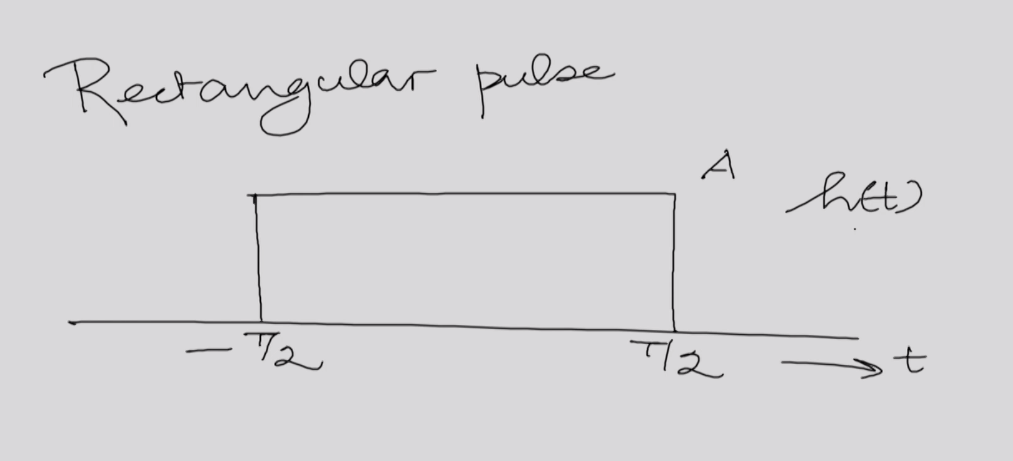
\includegraphics[width=12cm]{rectangularpulse.png}
		\caption{Symmetric Rectangular Pulse}
		\label{fig:rectangular_pulse}
	\end{figure}
	%%%
	Let us denote the Fourier transform by $ H(\Omega)$. Then
	\begin{equation}
		H(\Omega)=\int_{-\infty}^{\infty} \! {h(t) e^{-j\Omega t}} \ \dm t
	\end{equation}
	As $h(t)$ is zero except in the time interval $-T/2$ to $T/2$, we can write the above equation as
	\begin{equation}
		H(\Omega)=\int_{-T/2}^{T/2} \! {A e^{-j\Omega t}} \ \dm t =
		\frac{A e^{-j\Omega t}}{-j \Omega} \Bigg|_{-T/2}^{T/2}=
		\frac{A(e^{-j\Omega T/2}-e^{j\Omega T/2})}{-j\Omega}
		=\frac{AT (2j\sin({\Omega T/2}))}{j\Omega T}
	\end{equation}

	\begin{equation}
		H(\Omega)=\frac{AT\sin({\Omega T/2})}{\Omega T/2}
	\end{equation}
	And we can rewrite it as

	\begin{equation}
		H(f)=\frac{AT \sin({2\pi f T/2})}{2\pi f T/2}
	\end{equation}
	Where $f = \cfrac{\Omega}{2\pi}$ corresponds to the ${cycles}/{second}$ frequency, and $\Omega$ is of course the angular frequency.
	Now this expression also can be written as
	\begin{equation}
		H(\gamma)=\frac{AT \sin({\pi \gamma})}{\pi \gamma}
	\end{equation}
	Where $\gamma = f*T $.\\
	The function $\cfrac{\sin{\pi \gamma}}{\pi \gamma}$ is a very special function called a \emph{Sinc Function}. The sinc function in the form presented is often used in the context of signals and systems.

	\subsubsection{Sketch of the Sinc function}

		Here are the some properties of the Sinc function.
		\begin{itemize}
			\item It is an even function.
			\item It has nulls at every integer; so at 1, at 2, at 3 and so on, it will have value equal to zero.
			\item It tends to 1 as $\gamma$ tends to 0
			\item It is a damped sinusoid, i.e. the magnitude of oscillation decreases as $\gamma$ increases.
		\end{itemize}
		Using the above points we can sketch the Sinc function. So the sketch somewhat looks like Fig\ref{fig:sinc}.
		\begin{figure}[htp]
			\centering
			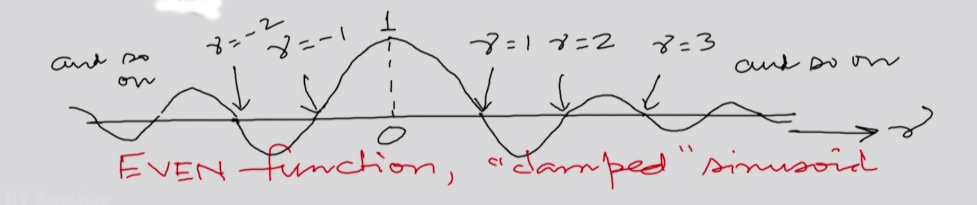
\includegraphics[width=12cm]{sinc.png}
			\caption{Sinc Function}
			\label{fig:sinc}
		\end{figure}

	\subsubsection{Important points regarding the Fourier transform of rectangular pulse}
		The pulse is limited in terms of its occupancy of the time axis. It goes only from  $-T/2$ to $+T/2$. On the other hand, the Fourier transform, in principle, lasts all over the frequency axis.
		What this means is that if we want to make a function vanish all over the time axis outside a certain finite interval, we have to bring together frequencies of all magnitudes and signs except for a few nulls.
		All these frequencies need to come together, in appropriate amplitudes, to form this rectangular pulse. Also note that the Fourier transform for this case is purely real. \\
		 When the pulse width is halved, the nulls of the Fourier transform are doubly spaced and the central amplitude is halved. This can be checked mathematically. We can see that Fig\ref{fig:pulse_FT_half}.
		\begin{figure}[htp]
			\centering
			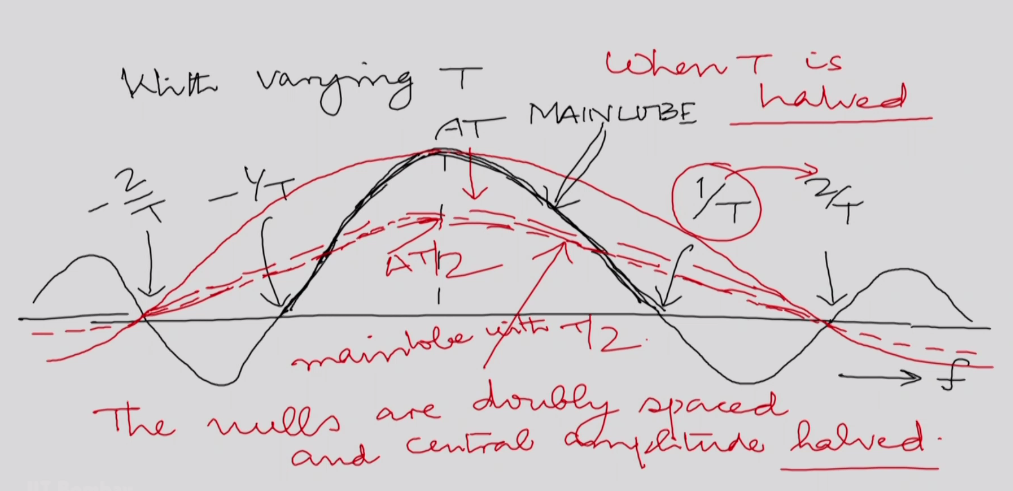
\includegraphics[width=12cm]{pulse_FT_half.png}
			\caption{Fourier Transform of Rectangular Pulse at width T and T/2 }
			\label{fig:pulse_FT_half}
		\end{figure}

\subsection{Properties of Fourier Transform}
	Let us see what happens to the Fourier transform when we change the original signal in some particular way.
	% When we change the signal in some way or when we bring signals together, what happens to the corresponding Fourier transform is what we will investigate in this section.
	\subsubsection{Linearity}
		Let $h_1(t)$ have the Fourier transform $H_1(\Omega)$ and let $h_2(t)$ have the Fourier transform $H_2(\Omega)$. Then, linearity says

		%\begin{equation}
		%$$\alpha h_1(t) + \beta h_2(t) \longrightarrow \alpha H_1(\Omega)+ \beta H_2(\Omega)$$
		%\end{equation}


		\[\alpha h_1(t) + \beta h_2(t) \xrightarrow{\mathcal{F}} \alpha H_1(\Omega)+ \beta H_2(\Omega)\]
		for all $\alpha$, $\beta$ $\in \mathbb{C}$ and all $h_1(t)$ and $h_2(t)$. Here, ${\mathcal{F}}$ means ``has the Fourier transform given by".

	\subsubsection{Proof of linearity}
		\begin{equation}
			 \alpha \{ H_1(\Omega) \} = \alpha \{ \int_{-\infty}^{\infty} \! h_1(t)e^{-j\Omega t} \ \dm t \}
			\label{eqn:one}
		\end{equation}

		\begin{equation}
			 \beta \{ H_2(\Omega) \} = \beta \{ \int_{-\infty}^{\infty} \! h_2(t)e^{-j\Omega t} \ \dm t \}
			\label{eqn:two}
		\end{equation}
		Add Eqn.\ref{eqn:one} and \ref{eqn:two}. We can write it as
		\begin{equation}
			\{ \alpha H_1(\Omega) + \beta H_2(\Omega) \} = \{ \int_{-\infty}^{\infty} \! (\alpha h_1(t) + \beta h_2(t))e^{-j\Omega t} \ \dm t \}
		\end{equation}

	\subsubsection{The Inverse Fourier transform}
		THe Inverse Fourier transform can be written as
		\begin{equation}
			H_1(\Omega) \xrightarrow{\mathcal{F}^{-1}} \frac{1}{2\pi} \int_{-\infty}^{\infty} \! H_1(t) e^{j\Omega t} \ \dm \Omega
		\end{equation}
		Note that $\Omega$ = $2\pi f$ and $d\Omega$= $2\pi df$. Hence,
		%%%
		\begin{equation}
			H_1(f) \xrightarrow{\mathcal{F^-1}} \int_{-\infty}^{\infty} \! H_1(f) e^{j2\pi ft} \ \dm f
		\end{equation}
		%%%
		Where $\Omega$ =  Radians/sec frequency
		And $f$ = cycles/sec frequency
		%%%
		\begin{itemize}
			\item We can clearly see that when frequency is in radians/sec then, we will have factor of $1/2\pi$ in the inverse Fourier transform and when frequency is in cycles/sec then the factor of $1/2\pi$ will not be there.
			\item In a way dealing with cycles/second frequency has some conveniences; we don't need to remember the factor of $1/2\pi$, or we can say, there is a perfect symmetry between the Fourier transform and the Inverse Fourier transform.
		\end{itemize}

	\subsubsection{Exercise}
		 Prove that linearity holds true for the inverse Fourier transform.

\subsection{Time Shift}
	What happens to the Fourier transform when we shift the signal in time? If
	\begin{equation}
		h(t) \xrightarrow{\mathcal{F}} H(\Omega)
	\end{equation}
	then, for a constant $\tau$,
	\begin{equation}
		h(t-\tau) \xrightarrow{\mathcal{F}} {?}
	\end{equation}
	%%%
	The Fourier transform would be
	\begin{equation}
		H(\Omega) =  \int_{-\infty}^{\infty} \! h(t-\tau) e^{-j\Omega t} \ \dm t
	\end{equation}
	Put $(t-\tau) = \lambda$  $\Rightarrow$  $t = \tau + \lambda$.
	So the Fourier transform is
	\begin{equation}
		H(\Omega) =  \int_{-\infty}^{\infty} \! h(\lambda) e^{-j\Omega (\lambda + \tau)} \ \dm \lambda =
		e^{-j\Omega \tau} \int_{-\infty}^{\infty} \! h(\lambda) e^{-j\Omega \lambda} \ \dm \lambda
	\end{equation}
	So,
	\begin{equation}
		h(t-\tau) \xrightarrow{\mathcal{F}} e^{-j\Omega \tau} H(\Omega)\   or\   e^{-j2\pi f\tau} H(f)
	\end{equation}
	Now it can be clearly seen that
	\begin{itemize}
		\item The magnitude of the Fourier transform is unchanged.
		\item The angle or the phase of the Fourier transform changes.
	\end{itemize}

	\subsubsection{Modulation}
		By modulation, we mean multiplying $h(t)$ by a rotating complex number (rotating with an angular velocity of $\Omega_0$). In this case, the Fourier transform is shifted by $\Omega_0$ forward.

		\begin{equation}
			e^{j\Omega_0 t} h(t) \xrightarrow{\mathcal{F}} {?}
		\end{equation}
		So the Fourier transform would be
		\begin{equation}
			 \int_{-\infty}^{\infty} \! e^{j\Omega_0 t} h(t) e^{-j\Omega t} \ \dm t =
			 \int_{-\infty}^{\infty} \! h(t) e^{-j(\Omega-\Omega_0) t} \ \dm t =
			 H(\Omega-\Omega_0)
		\end{equation}
		
		\begin{itemize}
			\item When we shift a function in time, it causes a modulation in the frequency domain (We remember, it multiplied the Fourier transform by a term $e^{-j\Omega \tau_0}$).

			\item When we modulate the function in time by multiplying by a rotating complex number, the corresponding Fourier transform shifts in frequency.

			\item Basically, shift in time becomes modulation in frequency, and modulation in time becomes a shift in frequency.
		\end{itemize}

	\subsubsection{Convolution Property of Fourier transform}
		The question to answer here is what will be the Fourier transform of $x_1(t)*x_2(t)$, given that the Fourier transforms of $x_1(t)$ and $x_2(t)$ are $X_1(\Omega)$ and $X_2(\Omega)$ respectively. 

		\begin{equation}
			x_1(t)\ast x_2(t) = \int_{-\infty}^{\infty}{x_1(\tau) x_2(t-\tau)}d\tau
		\end{equation}

		\begin{equation}
			x_1(t)\ast x_2(t) \xrightarrow{\mathcal{F}} {?}
		\end{equation}
		\noindent
		Now let's solve it. The Fourier transform can be written as
		\begin{equation}
			\int_{-\infty}^{\infty} \! \{ \int_{-\infty}^{\infty} \! x_1(\tau) x_2(t-\tau) \ \dm \tau \} e^{-j\Omega t} \ \dm t
		\end{equation}
		This is same as
		\begin{equation}
			\int_{-\infty}^{\infty} \! \int_{-\infty}^{\infty} \! x_1(\tau) x_2(t-\tau) e^{-j\Omega t} \ \dm \tau \dm t
		\end{equation}
		To solve the above double integral we will do a change of variables. Put
		\begin{equation}
			\alpha =\tau \ \text{and} \ \beta = (t-\tau)
		\end{equation}

		\begin{equation}
			\left( \begin{array}{c}
			\alpha \\
			\beta \end{array} \right)
			=
			\left( \begin{array}{cc}
			1 & 0 \\
			-1 & 1 \end{array} \right)
			\left( \begin{array}{c}
			\tau \\
			 t \end{array} \right)
		\end{equation}

		\begin{equation}
			\mathrm{d}\tau \mathrm{d}t = |\text{Det(transformation)}| \mathrm{d}\alpha \mathrm{d}\beta
		\end{equation}
		\noindent
		Hence,
		\begin{equation}
			\mathrm{d}\tau \mathrm{d}t = \mathrm{d}\alpha \mathrm{d}\beta
		\end{equation}
		Hence, the element of integration also remains the same because the Jacobian is $1$. Now the modified integral is
		
		\begin{equation}
			\int_{-\infty}^{\infty} \! \int_{-\infty}^{\infty} \! x_1(\alpha) x_2(\beta) \exp{-j\Omega(\alpha+\beta)} \ \dm \alpha \dm \beta
		\end{equation}
		
		\begin{equation}
			=\int_{-\infty}^{\infty} \! x_1(\alpha) \{ \int_{-\infty}^{\infty} \!
			x_2(\beta) e^{-j\Omega(\beta)} \ \dm \beta \} e^{-j\Omega \alpha} \ \dm \alpha
		\end{equation}
		This can be written as
		
		\begin{equation}
			X_2(\Omega) \int_{-\infty}^{\infty} \! x_1(\alpha) e^{-j\Omega \alpha} \ \dm \alpha
		\end{equation}
		So
		\begin{equation}
			x_1(t) \ast x_2(t) \xrightarrow{\mathcal{F}} X_1(\Omega)X_2(\Omega)
		\end{equation}
		\noindent
		Hence a convolution in the natural domain becomes a multiplication in the Fourier domain.

\subsection {Conclusion} In this section, we discussed about the Fourier transform of a rectangular pulse which is the ``Sinc function'', and its properties. We showed some of the properties of Fourier transform and their proofs.
\section{Module 2: Lecture 8\\Convolution Property of the Fourier Transform}

\subsection{Introduction}
	In this section, we will talk about the properties of the Fourier transform and specifically, we see more about the convolution property.
\subsection{Convolution Theorem}
	If two signals $x_1(t)$ and $x_2(t)$ both have Fourier transforms, which are $X_1(\Omega)$ and $X_2(\Omega)$ respectively, and if their convolution also has a Fourier transform, then this Fourier Transform is equal to the product of $X_1(\Omega)$ and $ X_2(\Omega)$.\\
	Mathematically,
	\begin{align}
		x_1(t) \xrightarrow{\mathcal{F}}& X_1(\Omega)\\
		x_2(t)\xrightarrow{\mathcal{F}}& X_2(\Omega)\\
		x_1(t)*x_2(t)\xrightarrow{\mathcal{F}}& X_1(\Omega).X_2(\Omega)
	\end{align}
	So, when we apply it to the context of LSI systems, we get
	\begin{equation}
		Y(\Omega)=X(\Omega)H(\Omega)
	\end{equation}
	where,
	\begin{align}
		x(t) &\xrightarrow{\mathcal{F}} X(\Omega)\\
		y(t) &\xrightarrow{\mathcal{F}} Y(\Omega)\\
		h(t) &\xrightarrow{\mathcal{F}} H(\Omega)
	\end{align}
	\begin{figure}[ht]
		\centering
		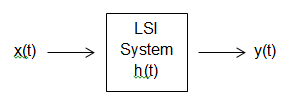
\includegraphics{fig0.png}
		%\caption{\label VVoltage generator (side view)}
	\end{figure}
	We said that there is a point-wise decoupling or memorylessness in the Fourier domain, meaning, the output at angular frequency $\Omega$ depends only on the input at angular frequency $\Omega$ and the impulse response at angular frequency $\Omega$ and none other.\\
	Where does this come from?\\
	$X(\Omega)$ is the component of input at angular frequency $\Omega$. Let us imagine $X(\Omega)e^{j\Omega t}$ as an input to the LSI system, where $X(\Omega)$ is a complex number.\\
	We have,
	\begin{figure}[h!]
		\centering
		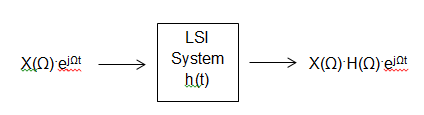
\includegraphics{fig1.png}
		%\caption{\label VVoltage generator (side view)}
	\end{figure}
	\begin{align}
		y(t) &= \int_{-\infty}^{\infty} \! h(\tau) X(\Omega) \ e^{j\Omega (t-\tau)} \ \dm \tau\\
		&= \left( \int_{-\infty}^{\infty} \! h(\tau) \ e^{-j\Omega \tau} \ \dm \tau \right) X(\Omega) \ e^{j\Omega t}\\
		&= X(\Omega) H(\Omega) \ e^{j\Omega t}
	\end{align}
	$H(\Omega)$ is the component of the impulse response along $e^{j\Omega t}$. Hence, $X(\Omega).H(\Omega)$ is the component of $y(t)$ along $e^{j\Omega t}$ and is equal to $Y(\Omega)$.\\
	\begin{equation}
		Y(\Omega)=X(\Omega).H(\Omega)
	\end{equation}
	%%%
	%%% CHECK THE FOLLOWING PART:
	This is analogous to an operator acting upon a force in mechanics. If $\nabla$ is the operator and if $\vec{F}$ the force vector such that
	\begin{equation}
	\vec{F}=F_x \hat{x} + F_y \hat{y} + F_z \hat{z}
	\end{equation}
	Then
	\begin{eqnarray}
	\nabla . \vec{F} &=& \nabla . (F_x \hat{x} + F_y \hat{y} + F_z \hat{z})\\
	\nabla . \vec{F} &=& \partial_x F_x \hat{x} + \partial_y F_y \hat{y} + \partial_z F_z \hat{z}\\
	\end{eqnarray}
	Similarly we resolve the input into its components along the different $\Omega$'s, i.e. $ej\Omega  t$.
	\begin{eqnarray}
	x(t)&=&\sum_i X(\Omega_i).\textrm{exp}(j\Omega_i t)\\
	y(t)&=&\sum _i X(\Omega_i).H(\Omega_i).\textrm{exp}(j\Omega_i t)
	\end{eqnarray}
	In a way, the idea is to decouple the action of the LSI system when we think of the input as comprising of different complex exponentials rotating at different angular frequencies, both positive and negative.
	%%%
	%%%
\subsection{What is a transform?}
	More generally, transform is a change of paradigm. Paradigm means world view. In a system point of view, a signal is a mapping from the independent variable to complex numbers, while a system is a mapping from signals to signals. Whereas a transform is a mapping of the signals and systems altogether to the transformed domain of signals and systems.
\subsection{Convolution or Multiplication}
	Doing multiplication, in general, is easier than convolution. To find the convolution, take Fourier transforms of the two signals, multiply them and then take its inverse Fourier transform.
	\begin{align}
		x_1(t) &\xrightarrow{\mathcal{F}} X_1(\Omega)\\
		x_2(t) &\xrightarrow{\mathcal{F}} X_2(\Omega)\\
		X_1(\Omega).X_2(\Omega) &\xrightarrow{\mathcal{F}^{-1}} x_1(t) \ast x_2(t)
	\end{align}
	It is beneficial only if the Fourier transform operations are easier to perform, otherwise it is not always better to go through the Fourier domain.\\
	For example, take $x_1(t)=x_2(t)$ as a rectangular pulse as shown in Fig\ref{fig:rectangular_pulse}.
	\begin{figure}[h!]\label{fig:rectangular_pulse}
		\centering
		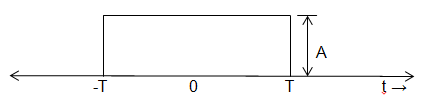
\includegraphics{fig2.png}
	\end{figure}
	Hence,
	\begin{align}
		X_1(\Omega)=X_2(\Omega) &= \int_{-\infty}^{\infty} \! x_1(t) \ e^{-j\Omega t} \ \dm t\\
		&= \int_{-T}^{T} \! A \ e^{-j\Omega t} \ \dm t\\
		&= \left(\frac{A}{-j\Omega} \ e^{-j\Omega t}\right) \Bigg|_{-T}^{T}\\
		&= \frac{2Aj \sin(\Omega t)}{j\Omega} \times \frac{T}{T}\\
		&= 2AT \frac{\sin{\Omega T}}{\Omega T}
	\end{align}
	Whereas the convolution leads to
	\begin{equation}
		x_1(t) \ast x_2(t)=\int_{-\infty}^{\infty} \! x_1(\tau)x_2(t-\tau) \ \dm \tau
	\end{equation}
	Now, $x_1(\tau) x_2(t-\tau)$ is non-zero only when some area of both the pulses coincide and is non- zero for that range only.
	This happens only for $t \in [-2T,2T]$
	\begin{figure}[h!]
	\centering
	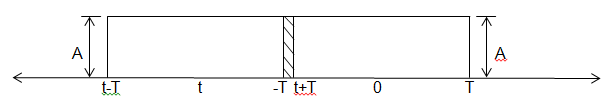
\includegraphics[scale=0.9]{fig3.png}
	\end{figure}
	Therefore, for $t \in [-2T,0]$
	\begin{align}
		x_1(t) \ast x_2(t) &= \int_{-\infty}^{\infty} \! x_1(\tau)x_2(t-\tau) \ \dm \tau\\
		&= \int_{-T}^{t+T} \! A^2 \ \dm \tau \\
		&= A^2 (t+2T)
	\end{align}
	and for $t \in [0,2T]$
	\begin{align}
		x_1(t) \ast x_2(t) &= \int_{-\infty}^{\infty} \! x_1(\tau)x_2(t-\tau) \ \dm \tau\\
		&= \int_{t-T}^{T} \! A^2 \ \dm \tau \\
		&= A^2 (2T-t)
	\end{align}
	\begin{figure}[ht]
		\centering
		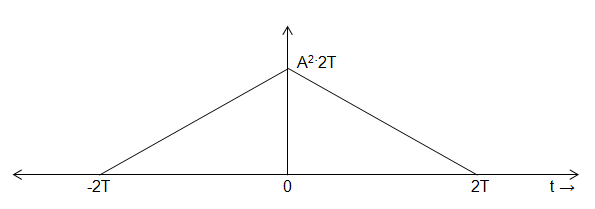
\includegraphics[scale=0.9]{fig4.png}
	\end{figure}
	Now the Fourier transform of $x_1(t)*x_2(t)$ is $X_1(\Omega)X_2(\Omega)$ which is equal to	
	\begin{equation}
		X_1(\Omega)X_2(\Omega) = \left( 2AT \frac{\sin(\Omega T)}{\Omega T} \right) ^2
	\end{equation}

\subsection{The Principle of Duality}

	We know that
	\begin{equation}
		X(\Omega) = \int_{-\infty}^{\infty} \! x(t) e^{-j\Omega t} \ \mathrm{d}t
	\end{equation}	
	and
	\begin{equation}
		x(t) = \frac{1}{2\pi}\int_{-\infty}^{\infty} \! X(\Omega) e^{j\Omega t} \ \mathrm{d}\Omega
	\end{equation}
	Now, in the second integral, let's interchange `$t$' and `$\Omega$'. Hence,
	\begin{equation}
		x(\Omega) = \frac{1}{2\pi}\int_{-\infty}^{\infty} \! X(t) e^{j\Omega t} \ \mathrm{d}t
	\end{equation}
	Hence,
	\begin{equation}
		x(-\Omega) = \frac{1}{2\pi}\int_{-\infty}^{\infty} \! X(t) e^{-j\Omega t} \ \mathrm{d}t
	\end{equation}
	Hence,
	\begin{equation}
		2\pi [x(-\Omega)] = \int_{-\infty}^{\infty} \! X(t) e^{-j\Omega t} \ \mathrm{d}t
	\end{equation}
	This shows that, if
	\begin{equation}
		x(t) \xrightarrow{\mathcal{F}} X(\Omega)
	\end{equation}
	then
	\begin{equation}\label{eqn:duality}
	X(t) \xrightarrow{\mathcal{F}} 2\pi [x(-\Omega)]
	\end{equation}
	This is the principle of duality for the Fourier transform. \\
	Let us take the example of the same rectangular pulse which we considered in the earlier section. The Fourier transform of the rectangular pulse is given by
	\begin{equation}
		X(\Omega) = 2AT \frac{\sin(\Omega T)}{\Omega T}
	\end{equation}
	Let us invoke duality here. We will replace $T$ by $W$ for convenience of notation Hence,
	\begin{equation}
		X(t) = 2AW \frac{\sin{(W t)}}{W t} \xrightarrow{\mathcal{F}} 2\pi [x(-\Omega)]
	\end{equation}
	Here, $2\pi x(\Omega)$ is the rectangular pulse with width $2W$ and height $2\pi A$. As the pulse is symmetric, $x(-\Omega) = x(\Omega)$.\\
	We can see why this is a very useful property. Say you want to evaluate the convolution of $\sin(Wt)/Wt$. It is very difficult to evaluate it using the direct expression of the convolution. But, we can invoke the principle of duality here. We know that the Fourier transform of a convolution is the product of their Fourier transforms. Hence, applying this to $X(t)$,
	\[
	X(t)*X(t) \xrightarrow{\mathcal{F}} [2\pi x(\Omega)]^2
	\]
	Now, it is very easy to evaluate the right hand side. It is in fact the same symmetric rectangular pulse, but with height $(2\pi A)^2$. Hence, it is equal to $(2\pi)^2 A x(\Omega)$. Therefore, we have,
	\begin{equation}\label{eqn:sinc_convolution}
	X(t)*X(t) \xrightarrow{\mathcal{F}} (2\pi)^2 A \ x(\Omega)
	\end{equation}
	Now, we know from the principle of duality (Eqn.\ref{eqn:duality}), that
	\begin{equation}
		X(t) \xrightarrow{\mathcal{F}} 2\pi [x(-\Omega)]
	\end{equation}
	Comparing this with Eqn.\ref{eqn:sinc_convolution}, we get,
	\begin{equation}
		X(t)*X(t) = 2\pi A \ X(t) = 2\pi A \left( 2AW \frac{\sin(Wt)}{Wt} \right)
	\end{equation}
	Hence, the evaluation of the convolution of $\sin(Wt)/Wt$ and other complicated functions with themselves can become a lot easier and straightforward if we invoke the principle of duality.

\section{Module 2: Lecture 9\\Multiplication Theorem and Parseval's Theorem}


\subsection{Introduction}
We have seen in the last few sessions, the property of duality and the convolution – multiplication parallel. We will now see the implications of duality, deriving what we call ‘Multiplication theorem’ and then its application called the ‘Parseval’s theorem’.

\subsection{Multiplication}
Let us take $x_1(t)$ and $x_2(t)$ with Fourier transforms $X_1(\Omega)$ and $X_2(\Omega)$ respectively. We derived earlier the Fourier transform of $x_1(t) \ast x_2(t)$ to be $X_1(\Omega)X_2(\Omega)$. We shall now try to find a general expression for the Fourier transform of the product $x_1(t)x_2(t)$.
\\
We have,            
\begin{equation}
x_1(t)\xrightarrow{\mathcal{F}} X_1(\Omega)
\end{equation}
\begin{equation}
x_2(t) \xrightarrow{\mathcal{F}} X_2(\Omega)
\end{equation}
\begin{equation}
x_1(t) \ast x_2(t)\xrightarrow{\mathcal{F}} X_1(\Omega)X_2(\Omega)
\end{equation}

Applying duality on (3) gives
\[
X_1(t)X_2(t)
\xrightarrow{\mathcal{F}}
2\pi (x1 \ast x2)(-\Omega)
\]
Also by duality,

\[
X_1(t)
\xrightarrow{\mathcal{F}}
2 \pi x_1(-\Omega)
\]
\[
X_2(t)
\xrightarrow{\mathcal{F}}
2 \pi x_2(-\Omega)
\]

$2\pi x_1(-\Omega) \ast x_2(-\Omega)$, which is the Fourier transform of $X_1(t)X_2(t)$, can be re-written as,
\[
\frac{1}{2\pi} ( 2\pi x_1(-\Omega) * 2\pi x_2(-\Omega) )
\]
Notice that $2\pi x_1(-\Omega)$ is the Fourier transform of $X_1(t)$ and $2\pi x_2(-\Omega)$ is the Fourier transform of $X_2(t)$.
Therefore we can see that the Fourier transform of the product $X_1(t)X_2(t)$ is the convolution of Fourier transforms of the individual time domain functions multiplied by a factor of $\frac{1}{2\pi}$. 

\subsubsection*{Theorem}
If 
\[
y_1(t)
\xrightarrow{\mathcal{F}} Y_1(\Omega)
\]
\[
y_2(t)
\xrightarrow{\mathcal{F}}
Y_2(\Omega)
\]
Then the Fourier transform the product (provided all the Fourier transforms exist) is,
\begin{equation}
y_1(t)y_2(t) 
\xrightarrow{\mathcal{F}}
\frac{1}{2\pi} 
( Y_1(\Omega) \ast Y_2(\Omega) )
\end{equation}
Multiplication of one signal by another can be thought of as using one signal to scale or modulate the amplitude of the other, and consequently, the multiplication of two signals is often referred to as 'amplitude modulation'. For this reason, (4) is sometimes referred to as the modulation property.


\subsubsection*{Special Case of Multiplication Theorem}
We have seen from the multiplication theorem, if $y_1(t)$ and $y_2(t)$ have the following Fourier transforms, 

\[
y_1(t)
\xrightarrow{\mathcal{F}}
Y_1(\Omega)
\]\[
y_2(t)
\xrightarrow{\mathcal{F}}
Y_2(\Omega)
\]
then
\[
y_1(t) y_2(t) 
\xrightarrow{\mathcal{F}}
\frac{1}{2\pi}
{ Y_1(\Omega) \ast Y_2(\Omega) }
\]
Let us find the Fourier transform of $y_1(t)\overline{y_2(t)}$:
We will first find out the Fourier transform of $\overline{y_2(t)}$ and then get the Fourier transform of $y_1(t)$ in two different ways:\begin{enumerate}
\item Using the multiplication theorem.
\item By the general definition of Fourier transform of any given function.
\end{enumerate}
First, the Fourier transform of  $\overline{y_2(t)}$:
The inverse Fourier transform of a given function $X(\Omega)$ is given by 
\[
x(t) = \frac{1}{2\pi}\int_{-\infty}^{\infty}{ X(\Omega) 
e^{j \Omega t}d\Omega }
\]
Taking the complex conjugate of the above,
\[	
\overline{x(t)} = \frac{1}{2\pi}\int_{-\infty}^{\infty}{\overline{X(\Omega)}e^{-j \Omega t}d\Omega }
\]  
Transforming $\Omega$ with $-\alpha$,
\begin{equation}
\overline{x(t)} = \frac{1}{2\pi}\int_{-\infty}^{\infty}{\overline{X(-\alpha)}e^{j \alpha t}d\alpha }
\end{equation}
From equation (5) we can observe that the Fourier transform of  $\overline{x(t)}$ is $\overline{X(-\alpha)}$.
Therefore 
\[
\overline{y_2(t)}
\xrightarrow{\mathcal{F}}
\overline{Y_2(-\Omega)}
\]
\noindent
From multiplication theorem, we can get the Fourier transform of the product $y_1(t)\overline{y_2(t)}$
\[
y_1(t)\overline{y_2(t)}
\xrightarrow{\mathcal{F}}
\frac{1}{2\pi} { 
Y_1(\Omega) 
\ast 
\overline{Y_2(-\Omega)}}\]
We can also obtain the Fourier transform using the general definition, i.e
\[
y_1(t)\overline{y_2(t)} \xrightarrow{\mathcal{F}}
\int_{-\infty}^{\infty}
{ y_1(t)\overline{y_2(t)} e^{-j\Omega t}dt }
\]

The Fourier transforms of $y_1(t)\overline{y_2(t)}$  obtained by either method should be identical, and hence we can write,
\[
\frac{1}{2\pi} { Y_1(\Omega)
 \ast \overline{Y_2(-\Omega)}} = 
\int_{-\infty}^{\infty}
{ y_1(t)\overline{y_2(t)} e^{-j\Omega t}dt }
\]

\[
\frac{1}{2\pi}
\int_{-\infty}^{\infty} \!
{Y_1(\Omega - \lambda)\overline{Y_2(-\lambda)}\ \mathrm{d}\lambda}
= 
\int_{-\infty}^{\infty}
{ y_1(t)\overline{y_2(t)} e^{-j\Omega t}dt }
\]

In the above equation, put $\Omega  =0$, the identity becomes
\[
\frac{1}{2\pi}
\int_{-\infty}^{\infty}
{Y_1(-\lambda)\overline{Y_2(-\lambda)}d\lambda}
= 
\int_{-\infty}^{\infty}
{ y_1(t)\overline{y_2(t)}dt }
\]

In the left hand side integral above, transform using $-\lambda \rightarrow \beta$, then
$d\lambda \rightarrow -d\beta$, and as $\lambda$ goes from $-\infty$ to $+\infty$, $\beta$ goes from $+\infty$ to $-\infty$. 
The equation becomes
\[
\frac{1}{2\pi} 
\int_{-\infty}^{\infty}
{ Y_1(\beta) 
\overline{Y_2(\beta)} d\beta } = \int_{-\infty}^{\infty}
{ y_1(t) \overline{y_2(t)}  dt } 
\]

Observe that the right hand side is essentially the inner product of $y_1(t)$ and $y_2(t)$  and the left hand side is the inner product of $Y_1(\Omega)$ and   $Y_2(\Omega)$ multiplied by a factor of $\frac{1}{2\pi}$.  Essentially, arrived at an equivalence between inner products in time domain and inner product in frequency domain. This is called the Parseval's theorem. 

\subsubsection*{Theorem}
If $y_1(t)$ and $y_2(t)$ have respectively their Fourier transforms $Y_1(\Omega)$ and $Y_2(\Omega)$, then the inner product of $y_1(t)$ and $y_2(t)$ is $\frac{1}{2\pi}$ times the inner product of $Y_1(\Omega)$ and $Y_2(\Omega)$
\[
\int_{-\infty}^{\infty}
{ y_1(t) \overline{y_2(t)} dt }  = \frac{1}{2\pi} 
\int_{-\infty}^{\infty}
{ Y_1(\Omega) \overline{Y_2(\Omega)} d\Omega }
\]









                



                     

\section{Module 2: Lecture 10\\Spectral Density}

\subsection{Introduction}
\noindent
In the previous lecture, we derived the multiplication property of the Fourier Transform which subsequently led to the derivation of Parseval’s Theorem. 
In this lecture, we will see more on the interpretation of the Parseval’s theorem as the invariance of the inner product of two signals calculated in time and angular frequency (or Fourier) domain. 
We will also define the energy of a signal and relate it with the Parseval’s Theorem and introduce the notion of Spectral Density of a signal.
Having done that, we will introduce the differentiation property of the Fourier Transform and its dual which will help us in calculating Fourier transforms of many more signals from the already known simpler Fourier transforms.
\subsection{Invariance of Inner Product on Change of Basis}
The property
\[
\int\limits_{-\infty}^{\infty}x(t)\overline{y(t)} dt = \cfrac{1}{2\pi}\int\limits_{-\infty}^{\infty}X(\Omega)\overline{Y(\Omega)} d\Omega
\]
has a deeper implication when we think of this in terms of the inner product of $x$ and $y$. Recall from vector algebra that in two dimensions, we can write any vector $\overrightarrow{v}$ as a linear combination of any two orthonormal basis vectors. Consider two such vectors, and two different sets of orthonormal vectors, such that
\[
\overrightarrow{v_1}=v_{11}\hat{u}_1+v_{12}\hat{u}_2 = v_{13}\hat{u}_3+v_{14}\hat{u}_4
\]
and
\[
\overrightarrow{v_2}=v_{21}\hat{u}_1+v_{22}\hat{u}_2 = v_{23}\hat{u}_1+v_{24}\hat{u}_4
\]
Now, the inner product or the dot product between the two vectors is the magnitude of one vector times the projection of the second vector along the first vector. The important thing to note here is that the inner product is a property of the vectors in themselves. This inner product, by definition, \emph{does not depend on which basis we choose to express them}. Thus,
\[
\overrightarrow{v_1}.\overrightarrow{v_2}=v_{11}v_{21}+v_{12}v_{22} = v_{13}v_{23}+v_{14}v_{24}
\]

This is exactly what the meaning of Parseval's theorem is. In the time domain, the basis vectors used, as you can remember from the first model, are the unit impulses:
\[
x(t) = \int_{-\infty}^{+\infty} \! x(\lambda)\delta(t-\lambda) \ \mathrm{d}\lambda
\]
Whereas in the frequency domain, the basis vectors are the rotating complex numbers or phasors:
\[
X(\Omega) = \int_{-\infty}^{+\infty} \! x(\lambda)e^{-j\Omega\lambda} \ \mathrm{d}\lambda
\]
But the inner product between two signals remains independent of the basis, which is what the Parseval's theorem states.
\[
\int\limits_{-\infty}^{\infty}x(t)\overline{y(t)}dt = \cfrac{1}{2\pi}\int\limits_{-\infty}^{\infty}X(\Omega)\overline{Y(\Omega)}d\Omega
\]
The factor of $2\pi$ arises due to the same reason why it arrived in the inverse Fourier transform, which is the normalization of the complex exponential.
\subsection{Energy of a Signal}
\noindent
The energy $E_x$ of a continuous time signal $x(t)$ is defined as

$$E_x = \int\limits_{-\infty}^{\infty}|x(t)|^2dt$$

\subsubsection{Relating Energy of a Signal and Parseval's Theorem}
\noindent
Consider two continuous time signals $x(t)$ and $y(t)$ with Fourier Transforms $X(\Omega)$ and $Y(\Omega)$ respectively. Then Parseval's theorem states that,

$$\int\limits_{-\infty}^{\infty}x(t)\overline{y(t)}dt = \cfrac{1}{2\pi}\int\limits_{-\infty}^{\infty}X(\Omega)\overline{Y(\Omega)}d\Omega$$

\noindent
where $(\cdot)^*$ denotes the complex conjugate of the corresponding signal.

\noindent
Now, if we substitute $y(t) = x(t)$ in the above relation, we get,

$$\int\limits_{-\infty}^{\infty}x(t)\overline{x(t)}dt = \cfrac{1}{2\pi}\int\limits_{-\infty}^{\infty}X(\Omega)\overline{X(\Omega)}d\Omega$$

\noindent
Since, $x(t)\overline{x(t)} = |x(t)|^2$ and $X(\Omega)\overline{X(\Omega)} = |X(\Omega)|^2$ we get,

$$\int\limits_{-\infty}^{\infty}|x(t)|^2dt = \cfrac{1}{2\pi}\int\limits_{-\infty}^{\infty}|X(\Omega)|^2d\Omega$$

\noindent
From the above relation, we see that the energy of a signal can also be calculate using the formula,

$$E_x = \cfrac{1}{2\pi}\int\limits_{-\infty}^{\infty}|X(\Omega)|^2d\Omega$$

\subsubsection{Energy Spectral Density}
\noindent
We have seen that if a signal $x(t)$ has a Fourier Transform $X(\Omega)$, its energy can be calculated from the angular frequency domain using the formula,

$$E_x = \cfrac{1}{2\pi}\int\limits_{-\infty}^{\infty}|X(\Omega)|^2d\Omega$$

\noindent
Integrating $|X(\Omega)|^2$ over the entire angular frequency axis and multiplying the result by $\cfrac{1}{2\pi}$ gives us the energy of the signal.

\noindent
Thus $|X(\Omega)|^2$ conveys the distribution of energy along the angular frequency axis.

\noindent
Hence, the integrand $|X(\Omega)|^2$ in the above formula is of significance and is called the Energy Spectral Density of the signal $x(t)$.

\subsubsection{Energy Spectral Density and Linear Shift-Invariant Systems}
\noindent
Consider a linear shift invariant system having an impulse response $h(t)$ and let $y(t)$ be the output  of this system when an input $x(t)$ is applied to it.

\noindent
Then, we have

$$y(t) = x(t)*h(t)$$

\noindent
where $*$ denotes the convolution operator.

\noindent
Assume that the Fourier transforms of $h(t)$ and $x(t)$. Let $H(\Omega)$ and $X(\Omega)$ be their respective Fourier Transforms.

\noindent
Then the Fourier Transform $Y(\Omega)$ of the signal $y(t)$ is given by.

$$Y(\Omega) = X(\Omega)H(\Omega)$$

\noindent
Therefore,

$$|Y(\Omega)|^2 = |X(\Omega)|^2|H(\Omega)|^2$$

\noindent
Note that $|Y(\Omega)|^2$, $|X(\Omega)|^2$ and $|H(\Omega)|^2$ are essentially the energy spectral densities of the signals $y(t)$, $x(t)$ and the impulse response $h(t)$ respectively.

\noindent
Thus, the energy spectral density of the output is equal to the energy density of the input multiplied by the energy density of the frequency response.

\subsection{The Differentiation Property of the Fourier Transform}


\noindent
Consider a continuous time signal $x(t)$ which has a Fourier transform $X(\Omega)$ then we can write,

$$x(t) = \cfrac{1}{2\pi}\int\limits_{-\infty}^{\infty}X(\Omega)e^{j\Omega t}d\Omega$$

\noindent
Differentiating on both sides with respect to $'t'$ we get,

$$\cfrac{dx(t)}{dt} = \cfrac{d}{dt}\left(\cfrac{1}{2\pi}\int\limits_{-\infty}^{\infty}X(\Omega)e^{j\Omega t}d\Omega\right)$$

\noindent
Taking the derivative under the integral we get,

$$\cfrac{dx(t)}{dt} = \cfrac{1}{2\pi}\int\limits_{-\infty}^{\infty}X(\Omega)\cfrac{de^{j\Omega t}}{dt}d\Omega$$

\noindent
Therefore,

$$\cfrac{dx(t)}{dt} = \cfrac{1}{2\pi}\int\limits_{-\infty}^{\infty}(X(\Omega)j\Omega)e^{j\Omega t}d\Omega$$

\noindent
Comparing the above equation with the definition of the inverse Fourier Transform, we see that for the signal $x(t)$ has the Fourier Transform $j\Omega X(\Omega)$.

\noindent
Thus, the differentiation property of the Fourier transform states that if a continuous variable signal $x(t)$ has the Fourier Transform $X(\Omega)$, then the Fourier transform of $\cfrac{dx(t)}{dt}$ is $j\Omega X(\Omega)$.

\subsubsection{Interpretation of the differentiation property}
\noindent
The differentiation property of the Fourier Transform can be interpreted in the following way: If you differentiate a signal $x(t)$ with respect to $t$, then the Fourier transform $X(\Omega)$ gets phase shifted by $90$ degrees and scaled by $\Omega$.

\subsubsection{Duality and the differentiation property}
\noindent
We can see that there are two operators involved in the differentiation property - differentiation in time domain and pointwise multiplication by $j\Omega$ in angular frequency domain.
But, what changes happens to the signal $x(t)$ when we differentiate the Fourier Transform $X(\Omega)$ with respect to $\Omega$ in angular frequency domain? Let's find out

\noindent
We know that,

$$X(\Omega) = \int\limits_{-\infty}^{\infty}x(t)e^{-j\Omega t}dt$$

\noindent
Differentiating both the sides with respect to $\Omega$ we get,

$$\cfrac{dX(\Omega)}{d\Omega} = \cfrac{d\int\limits_{-\infty}^{\infty}x(t)e^{-j\Omega t}dt}{d\Omega}$$

\noindent
Taking the derivative under the integral we get, 

$$\cfrac{dX(\Omega)}{d\Omega} = \int\limits_{-\infty}^{\infty}x(t)\cfrac{de^{-j\Omega t}}{d\Omega}dt$$

\noindent
Therefore,


$$\cfrac{dX(\Omega)}{d\Omega} = \int\limits_{-\infty}^{\infty}-jtx(t)e^{-j\Omega t}dt$$


\noindent
Comparing the above equation with the definition of the Fourier Transform we see that Fourier transform of $-jtx(t)$ is $\cfrac{dX(\Omega)}{d\Omega}$.

\noindent
Thus, differentiation of Fourier Transform $X(\Omega)$ with respect to $\Omega$ in angular frequency domain leads to pointwise multiplication of signal $x(t)$ by $-jt$ in the time domain. Hence, the above property is the dual of the differentiation property.

\noindent
Differentiation in one domain leads to pointwise multiplication in the other domain and pointwise multiplication in one domain leads to differentiation in the other domain. This is the duality property of the Fourier Transform.








\end{document}